% Сборка: xelatex -jobname=defense_notes --aux-directory=build --output-directory=output/pdf main.tex
\documentclass[12pt,a4paper]{article}
\usepackage{fontspec,polyglossia}
\setdefaultlanguage{russian}
\setotherlanguage{english}
\setmainfont{Times New Roman}[Ligatures=TeX]
\newfontfamily\cyrillicfont{Times New Roman}[Script=Cyrillic,Ligatures=TeX]
\setmonofont{Courier New}
\newfontfamily\cyrillicfonttt{Courier New}[Script=Cyrillic]
\usepackage[left=25mm,right=20mm,top=20mm,bottom=20mm]{geometry}
\usepackage{amsmath,amssymb,amsthm,mathtools,bm}
\usepackage{microtype,indentfirst,setspace}
\setstretch{1.12}
\setlength{\parindent}{1.1cm}
\setlength{\parskip}{3pt}
\setlength{\abovedisplayskip}{7pt}
\setlength{\belowdisplayskip}{7pt}
\setlength{\abovedisplayshortskip}{4pt}
\setlength{\belowdisplayshortskip}{4pt}
\usepackage{booktabs,tabularx,longtable,array,enumitem}
\setlist{nosep,topsep=4pt,leftmargin=*}
\renewcommand{\arraystretch}{1.15}
\newcolumntype{Y}{>{\raggedright\arraybackslash}X}
\usepackage{graphicx,titlesec,fancyhdr}
\makeatletter
\newenvironment{guidefigure}{\par\addvspace{6pt}\noindent
  \begin{minipage}{\textwidth}\def\@captype{figure}\centering
}{\end{minipage}\par\vspace{6pt}}
\makeatother
\titleformat{\section}{\large\bfseries}{\thesection}{0.7em}{}
\titleformat{\subsection}{\normalsize\bfseries}{\thesubsection}{0.7em}{}
\titleformat{\subsubsection}{\normalsize\bfseries}{\thesubsubsection}{0.7em}{}
\setcounter{tocdepth}{2}
\numberwithin{equation}{section}
\DeclareMathOperator{\sgn}{sgn}
\DeclareMathOperator{\sat}{sat}
\DeclareMathOperator{\rank}{rank}
\newcommand{\norm}[1]{\left\lVert#1\right\rVert}
\newcommand{\lecture}[2]{\par\noindent\textit{Лекция #1, слайды #2.}\par}
\newcommand{\addition}{\par\noindent\textbf{Дополнение для защиты.} }
\pagestyle{fancy}
\fancyhf{}
\fancyfoot[C]{\thepage}
\renewcommand{\headrulewidth}{0pt}
\usepackage[unicode,colorlinks=true,linkcolor=black,urlcolor=black]{hyperref}
\hypersetup{pdftitle={Нелинейные системы управления Подготовка к защите работ 3 4 и 5},pdfauthor={}}
\raggedbottom
\emergencystretch=2em
\widowpenalty=10000
\clubpenalty=10000
\brokenpenalty=10000

\begin{document}
\begin{center}
  {\LARGE\bfseries Нелинейные системы управления\par}
  \vspace{5mm}
  {\large Подготовка к защите лабораторных работ 3 4 и 5\par}
\end{center}

Конспект объединяет теорию шести лекций и пошаговый разбор лабораторных
работ. После изучения нужно уметь объяснить выбор регулятора, вывести его
формулу, назвать область определения и доказать именно тот вид устойчивости,
который заявлен в решении. Формулы без условий применимости для защиты
недостаточны.

Сначала разберите постановку стабилизации и метод Ляпунова, затем переходите
к линеаризации обратной связью, бэкстеппингу и скользящему режиму. В каждом
разборе работы сначала восстановите вычисления самостоятельно, затем
сопоставьте их с решением. Последний раздел содержит вопросы для устного
повторения.

\begin{center}
\begin{tabularx}{\textwidth}{@{}lYr@{}}
\toprule
Файл & Содержание & Слайдов\\
\midrule
\texttt{L2.pdf} & Стабилизация обратной связью, линеаризация, интегральное управление & 47\\
\texttt{L3.pdf} & Устойчивость, функции Ляпунова, ЛаСалль, ISS, каскады & 44\\
\texttt{L4\_1.pdf} & Линеаризация обратной связью и ошибки модели & 29\\
\texttt{L4\_2.pdf} & Относительная степень, нормальная форма, нуль-динамика & 12\\
\texttt{L5.pdf} & Бэкстеппинг и системы строгой обратной связи & 27\\
\texttt{L6.pdf} & Скользящие режимы, адаптивное и робастное управление & 25\\
\bottomrule
\end{tabularx}
\end{center}

Ссылки на слайды относятся к номеру страницы соответствующего PDF.
Последовательные слайды, постепенно дополняющие одну формулу, объединены
в полный вывод. Обозначения сохранены по лекциям; дополнительные пояснения
и необходимые для работ результаты отмечены отдельно. В разных темах одна
буква может иметь разный смысл: например, $\gamma$ обозначает закон обратной
связи, входной коэффициент или коэффициент адаптации. Смысл каждый раз
задаётся локальным определением.

\tableofcontents
\clearpage
\section{Постановка задачи стабилизации}
\label{sec:foundations}

\subsection{Обратная связь по состоянию и по выходу}
\lecture{L2}{3--9}

Состояние $x\in\mathbb R^n$ содержит переменные, достаточные для описания
дальнейшего движения системы. Вход $u$ выбирает регулятор. Для объекта
\[
  \dot x=f(x,u)
\]
задача стабилизации состоит в построении закона управления, при котором
выбранное равновесие замкнутой системы асимптотически устойчиво.
Нужно обеспечить и малость отклонений при малых начальных возмущениях,
и их стремление к нулю со временем.

\textbf{Статическая обратная связь по состоянию} имеет вид
\[
  u=\gamma(x),\qquad \dot x=f\bigl(x,\gamma(x)\bigr).
\]
Слово «статическая» означает отсутствие собственной памяти регулятора.
Это не означает, что управление постоянно: оно изменяется вместе с $x(t)$.
Перед анализом устойчивости необходимо проверить
$f(0,\gamma(0))=0$. Во всех работах измеряется весь вектор состояния,
поэтому именно такая обратная связь непосредственно реализуема.

\textbf{Динамическая обратная связь} содержит собственное состояние $z$:
\[
  u=\gamma(x,z),\qquad \dot z=g(x,z).
\]
Пример собственной памяти --- накопленная ошибка интегрального регулятора.
Анализировать нужно уже объединённую систему $(x,z)$, а не только объект.
Если целевое равновесие регулятора выбрано нулевым, требование стабилизации
формулируется для $(x,z)=(0,0)$.

При \textbf{обратной связи по выходу} измеряется $y=h(x,u)$, а полный $x$
может быть неизвестен. Статический регулятор использует $u=\gamma(y)$;
динамический --- $u=\gamma(y,z)$ и уравнение для $z$, зависящее от доступных
измерений. Если в правой части этого уравнения непосредственно используется
неизмеряемый $x$, это уже не реализуемая обратная связь только по выходу.
В рассматриваемых работах такой проблемы нет: состояние измеряется целиком.

\addition Если $h$ зависит от $u$, подстановка $u=\gamma(y)$ может создать
алгебраическое уравнение относительно $u$. Нужно отдельно проверить его
разрешимость. В работе 3 выходы заданы как $y=h(x)$, поэтому этой
дополнительной трудности нет.

\subsection{Стабилизация ненулевого равновесия}
\lecture{L2}{10--13}

Равновесие --- состояние, которое можно поддерживать постоянным входом:
\begin{equation}
  f(x_{ss},u_{ss})=0.
  \label{eq:equilibrium-general}
\end{equation}
Задать желаемое $x_{ss}$ недостаточно: необходимо найти совместимое $u_{ss}$.
Если равенство~\eqref{eq:equilibrium-general} не выполняется, точка не является
равновесием и обычное требование её асимптотической устойчивости некорректно.

Вводятся отклонения, обозначенные в лекции индексом $\delta$:
\[
  x_\delta=x-x_{ss},\qquad u_\delta=u-u_{ss}.
\]
Для постоянного задания $\dot x_{ss}=0$, поэтому
\[
  \dot x_\delta=f(x_{ss}+x_\delta,u_{ss}+u_\delta)
  \equiv f_\delta(x_\delta,u_\delta),\qquad f_\delta(0,0)=0.
\]
Если синтезирован закон $u_\delta=\gamma(x_\delta)$, в исходных координатах
нужно записать
\begin{equation}
  u=u_{ss}+\gamma(x-x_{ss}).
  \label{eq:equilibrium-feedback}
\end{equation}
В этой формуле слева стоит полный вход $u$, а не отклонение $u_\delta$.

Для выходного задания сначала выбирают равновесие, удовлетворяющее
$h(x_{ss},u_{ss})=y_{ss}$, затем вводят
\[
  y_\delta=y-h(x_{ss},u_{ss})
  =h(x_{ss}+x_\delta,u_{ss}+u_\delta)-h(x_{ss},u_{ss}).
\]
Нулевой выход сам по себе не определяет единственное состояние:
разные внутренние состояния могут давать одинаковый $y$. Именно поэтому
в работе 3 понадобится анализ нуль-динамики.

\addition В третьей системе работы 4 при $x=0$ первая производная равна
$\dot x_1=\cos0=1$ независимо от $u$. Начало координат стабилизировать нельзя.
Выбрано совместимое равновесие $x_{ss}=(0,1,0,0)^T$, $u_{ss}=0$.
На графике нужно смотреть на $x_2-1$, а не требовать $x_2\to0$.

\subsection{Стабилизация по линейному приближению}
\lecture{L2}{14--17}

Пусть начало координат --- равновесие и $f$ непрерывно дифференцируема.
Матрицы линейного приближения определяются в точке равновесия:
\[
  A=\left.\frac{\partial f}{\partial x}\right|_{x=0,u=0},\qquad
  B=\left.\frac{\partial f}{\partial u}\right|_{x=0,u=0}.
\]
Тогда $\dot x=Ax+Bu$ описывает только первый порядок разложения исходного
объекта. Выбирают $u=-Kx$ так, чтобы $A-BK$ была гурвицевой:
\[
  \operatorname{Re}\lambda_i(A-BK)<0\quad\text{для всех }i.
\]
Производная правой части нелинейной замкнутой системы в нуле равна $A-BK$.
Из теоремы о линеаризации следует локальная экспоненциальная устойчивость
исходной системы. Слово «локальная» существенно: отброшенные нелинейности
могут стать определяющими вдали от равновесия.

\addition Пара $(A,B)$ управляема, если
\[
  \rank\begin{pmatrix}B&AB&\cdots&A^{n-1}B\end{pmatrix}=n.
\]
Тогда линейной обратной связью можно назначить все полюса. Для одной лишь
стабилизации достаточно стабилизируемости: все неуправляемые моды должны
уже иметь отрицательные действительные части. Неуправляемую неустойчивую
моду обратная связь по этому входу устранить не сможет.

Пример различия локального и глобального вывода:
$\dot x=x^3+u$, $u=-x$ дают $\dot x=-x+x^3$.
Линеаризация $\dot x=-x$ устойчива, но при $x>1$ правая часть положительна.
Регулятор стабилизирует нуль локально; глобального результата нет.

\subsection{Маятник и заданный угол}
\lecture{L2}{18--25}

В лекции рассматривается модель
\[
  \ddot\theta=-a\sin\theta-b\dot\theta+cT,
  \qquad a>0,\quad b\ge0,\quad c>0.
\]
Для постоянного угла $\theta=\delta$ скорость и ускорение равны нулю.
Отсюда находятся удерживающий момент и отклонения:
\[
  T_{ss}=\frac{a}{c}\sin\delta,\qquad
  x_1=\theta-\delta,\quad x_2=\dot\theta,\quad u=T-T_{ss}.
\]
В этих координатах
\[
  \dot x_1=x_2,\qquad
  \dot x_2=-a\bigl[\sin(x_1+\delta)-\sin\delta\bigr]-bx_2+cu.
\]
Обратите внимание на скобки: $\sin(x_1+\delta)-\sin\delta$ обращается в нуль
при $x_1=0$. Замена этого выражения на $\sin x_1+\delta-\sin\delta$
изменила бы модель.

Матрицы и матрица замкнутой системы равны
\[
  A=\begin{pmatrix}0&1\\-a\cos\delta&-b\end{pmatrix},\qquad
  B=\begin{pmatrix}0\\c\end{pmatrix},\qquad K=\begin{pmatrix}k_1&k_2\end{pmatrix},
\]
\[
  A-BK=\begin{pmatrix}0&1\\-(a\cos\delta+ck_1)&-(b+ck_2)\end{pmatrix}.
\]
Характеристический полином имеет вид
\[
  p(s)=s^2+(b+ck_2)s+a\cos\delta+ck_1.
\]
Для второго порядка гурвицевость эквивалентна положительности обоих
коэффициентов после старшего:
\[
  k_1>-\frac{a\cos\delta}{c},\qquad k_2>-\frac bc.
\]
Итоговый закон записывается через измеряемые угол и скорость:
\begin{equation}
  T=\frac{a}{c}\sin\delta-k_1(\theta-\delta)-k_2\dot\theta.
\end{equation}
Первое слагаемое удерживает равновесие, второе возвращает угол к заданию,
третье создаёт демпфирование. Даже для верхнего положения, где
$\cos\delta<0$, достаточно сильная позиционная обратная связь делает
линейное приближение устойчивым. Гарантия пока остаётся локальной.

\addition Если задан желаемый полином $s^2+d_1s+d_0$ с $d_0,d_1>0$, то
$k_1=(d_0-a\cos\delta)/c$, $k_2=(d_1-b)/c$.
Так выводится выбор коэффициентов, а не просто угадывается знак $K$.

\subsection{Линейный динамический регулятор по выходу}
\lecture{L2}{26--28}

Для $y=h(x)$ линейный выход имеет вид $y=Cx$, где
$C=\left.\partial h/\partial x\right|_0$.
Предполагаются стабилизируемость $(A,B)$ и обнаруживаемость $(A,C)$.
Обнаруживаемость означает, что все ненаблюдаемые моды уже устойчивы.
Линейный динамический регулятор лекции записан так:
\[
  \dot z=Fz+Gy,\qquad u=Lz+My.
\]
После подстановки в объект анализируется расширенная система
\begin{equation}
  \begin{pmatrix}\dot x\\\dot z\end{pmatrix}
  =\begin{pmatrix}A+BMC&BL\\GC&F\end{pmatrix}
   \begin{pmatrix}x\\z\end{pmatrix}.
\end{equation}
Требуется гурвицевость всей блочной матрицы. Устойчивость одной только
матрицы $F$ ничего не говорит об устойчивости взаимодействия регулятора
с объектом. При гладкости нелинейного объекта гурвицевость расширенного
линейного приближения даёт локальную устойчивость полного замкнутого контура.

\addition Наблюдатель даёт понятную реализацию этого подхода:
\[
  \dot z=Az+Bu+H(y-Cz),\qquad u=-Kz.
\]
Здесь $z$ --- оценка состояния; $H$ выбирается так, чтобы $A-HC$ была
гурвицевой. Ошибка $x-z$ удовлетворяет $\frac{d}{dt}(x-z)=(A-HC)(x-z)$.
Полюса линейного контура состоят из полюсов $A-BK$ и $A-HC$.
В лабораторных 3--5 наблюдатель не нужен, поскольку всё состояние измеримо.

\subsection{Статическая ошибка и интегральное управление}
\lecture{L2}{29--46}

Удерживающее воздействие $T_{ss}=a\sin\delta/c$ требует точных $a,c$.
Если вместо них использованы номинальные $a_0,c_0$, получается закон
\[
  T=\frac{a_0}{c_0}\sin\delta-k_1(\theta-\delta)-k_2\dot\theta.
\]
В установившемся режиме действительного объекта выполняется
\begin{equation}
  a\sin\theta_{ss}
  =c\frac{a_0}{c_0}\sin\delta-ck_1(\theta_{ss}-\delta).
  \label{eq:static-error-pendulum}
\end{equation}
Из этого уравнения в общем случае не следует $\theta_{ss}=\delta$.
Устойчивая система может остановиться с ненулевой статической ошибкой:
устойчивость равновесия и точность задания являются разными требованиями.

На схемах лекции в объекте стоят два интегратора: ускорение интегрируется
в скорость, скорость --- в угол. Позиционная ошибка и скорость возвращаются
с отрицательными знаками через $k_1,k_2$. Канал $a_0\sin\delta/c_0$ подаёт
номинальный удерживающий момент напрямую и сам по себе ошибки модели
не компенсирует.

В иллюстрации лекции коэффициент при $\sin\theta$ в объекте увеличивается
вдвое, задание равно $45^\circ$, а коэффициенты выбраны
$K=\begin{pmatrix}3a/c&a\end{pmatrix}$.
На графике без дополнительного интегратора
угол устанавливается примерно на $36^\circ$. С интегральным каналом
установившийся угол достигает $45^\circ$, хотя переходный процесс имеет
большее перерегулирование. Поэтому улучшение точности не означает
автоматического улучшения всех показателей переходного процесса.

Для устранения постоянной ошибки вводится
\[
  e=\theta-\delta,\qquad z=\int_0^t e(\tau)\,d\tau,\qquad \dot z=e.
\]
Закон лекции содержит интегральное слагаемое с единичным коэффициентом:
\begin{equation}
  T=T_{ss,0}-k_1e-k_2\dot\theta-z,
  \qquad T_{ss,0}=\frac{a_0}{c_0}\sin\delta.
\end{equation}
Если замкнутая система сходится к постоянному равновесию, условие
$\dot z=0$ требует $e=0$. Состояние интегратора при этом становится
$z_{ss}=T_{ss,0}-a\sin\delta/c$: оно накапливает недостающую постоянную
компенсацию. В номинальной модели $z_{ss}=0$.

\addition Интегратор нужно включать в анализ устойчивости. Для отклонений
$(e,\dot\theta,z-z_{ss})$ характеристический полином равен
\[
  p(s)=s^3+(b+ck_2)s^2+(a\cos\delta+ck_1)s+c.
\]
Кроме положительности коэффициентов, критерий Гурвица третьего порядка
требует
\[
  (b+ck_2)(a\cos\delta+ck_1)>c.
\]
Следовательно, механическое добавление интегратора к любому устойчивому
регулятору может сделать контур неустойчивым. Сначала выбирают коэффициенты,
затем проверяют расширенную систему.

Интегральная компенсация постоянной ошибки не равнозначна точному
подавлению произвольного неизвестного $h(t)$ из работы 5. Для переменного
возмущения потребуется отдельный анализ; лекционный непрерывный регулятор
маятника в работе 5 гарантирует малую окрестность нуля.

\subsection{Что нужно различать перед выбором метода}

\begin{center}
\begin{tabularx}{\textwidth}{@{}lYY@{}}
\toprule
Вопрос & Что проверяется & Типичная ошибка\\
\midrule
Равновесие & $f(x_{ss},u_{ss})=0$ & Требовать стабилизацию недостижимой точки\\
Устойчивость & Движение при начальных отклонениях & Считать достаточным один удачный график\\
Точность & Значение ошибки после переходного процесса & Принимать устойчивость за отсутствие ошибки\\
Измеримость & Какие переменные доступны регулятору & Использовать неизвестный параметр в реальном законе\\
Область гарантии & Локальная область или всё пространство & Называть локальную линеаризацию глобальным методом\\
\bottomrule
\end{tabularx}
\end{center}

\clearpage
\section{Устойчивость и метод Ляпунова}
\label{sec:stability}

\subsection{Что именно требуется доказать об устойчивости}
\label{subsec:stability-definitions}
\noindent\textit{Источник: L3, слайды 1--10.}

Лекция посвящена анализу устойчивости с помощью функции Ляпунова.
Для линейных систем в ней перечислены критерии Рауса--Гурвица,
Найквиста и Михайлова; для нелинейных --- круговой критерий,
критерий Попова и метод функций Ляпунова. Сами частотные критерии
в L3 не выводятся. Метод А. М. Ляпунова позволяет исследовать
устойчивость без явного решения дифференциальных уравнений.

Рассмотрим систему и её равновесие
\[
 \dot x=f(x),\qquad x(t_0)=x_0\in\mathbb R^n,\qquad f(0)=0.
\]
Здесь $x^*=0$ --- состояние, которое должно сохраняться при
отсутствии отклонений. Определения отвечают на разные вопросы.
\begin{enumerate}[leftmargin=*,itemsep=3pt]
 \item \textbf{Устойчивость по Ляпунову:} достаточно малое начальное
 отклонение остаётся малым при всех последующих временах:
 \[
  \forall\varepsilon>0\ \forall t_0\ge0\ \exists\delta(\varepsilon,t_0)>0:
  \quad \norm{x_0}<\delta\ \Longrightarrow\
  \norm{x(t)}<\varepsilon\quad\forall t\ge t_0.
 \]
 Сходимость к нулю здесь не требуется. На рисунке слайда 6
 траектория остаётся внутри трубки радиуса $\varepsilon$, хотя
 может колебаться и не приближаться к оси.
 \item \textbf{Асимптотическая устойчивость:} устойчивость по Ляпунову
 дополняется притяжением некоторой окрестности:
 \[
  \exists\delta_a>0:\quad \norm{x_0}<\delta_a
  \ \Longrightarrow\ \lim_{t\to\infty}x(t)=0.
 \]
 Поэтому одного наблюдения $x(t)\to0$ недостаточно: требуется
 также устойчивость.
 \item \textbf{Равномерность} означает независимость соответствующих
 оценок от начального момента $t_0$. \textbf{Глобальность}
 означает, что область притяжения охватывает всё пространство
 начальных состояний. Это разные свойства: первое относится
 ко времени начала движения, второе --- к величине $x_0$.
 \item \textbf{Экспоненциальная устойчивость} задаёт скорость
 затухания: существуют $c\ge1$, $\sigma>0$ и окрестность нуля, где
 \[
  \norm{x(t)}\le c\,e^{-\sigma(t-t_0)}\norm{x_0},\qquad t\ge t_0.
 \]
 При выполнении оценки для всех $x_0\in\mathbb R^n$ устойчивость
 глобально экспоненциальная.
 \item \textbf{Устойчивость за конечное время (finite-time):}
 равновесие устойчиво и для каждого допустимого $x_0$ существует
 конечное время установления $T(x_0)$, после которого
 \[
  x(t)=0\quad\forall t\ge t_0+T(x_0).
 \]
 \item \textbf{Устойчивость за фиксированное время (fixed-time):}
 дополнительно существует общая граница
 \[
  T(x_0)\le T_{\max}<\infty\quad\forall x_0\in\mathbb R^n.
 \]
 В первом случае время может неограниченно расти с $\norm{x_0}$,
 во втором одна оценка действует для всех начальных состояний.
\end{enumerate}

\textbf{Дополнение для защиты.}
Для автономной системы сдвиг $t_0$ не меняет уравнение, поэтому
обычные локальные определения устойчивости и асимптотической
устойчивости дают равномерность по $t_0$.
На слайде 8 экспоненциальная оценка записана сокращённо как
$\norm{x(t)}\le ce^{-\sigma t}$; в стандартной равномерной оценке
необходимы множитель $\norm{x_0}$ и время $t-t_0$, как выше.
Для равновесия $x^*\ne0$ все определения применяются к
отклонению $x-x^*$.

\subsection{Прямой метод Ляпунова: условия и геометрический смысл}
\label{subsec:stability-direct}
\noindent\textit{Источник: L3, слайды 2, 11--17.}

Пусть $D\subset\mathbb R^n$ --- открытая область, содержащая нуль,
а $f:D\to\mathbb R^n$ локально липшицева.
Это означает, что около каждой точки существует конечная
константа $L$, для которой
\[
 \norm{f(x)-f(y)}\le L\norm{x-y}.
\]
График на слайде 12 иллюстрирует ограниченность локального наклона:
не требуется ни глобальная константа $L$ на всём пространстве,
ни линейность $f$.

Ищем непрерывно дифференцируемую скалярную функцию
$V:D\to\mathbb R$, положительно определённую относительно нуля:
\[
 V(0)=0,\qquad V(x)>0\quad\text{при }x\in D\setminus\{0\}.
\]
Она играет роль обобщённой энергии. Её производная вычисляется
\emph{вдоль решений рассматриваемой системы}:
\[
 \dot V(x)=\sum_{i=1}^{n}\frac{\partial V}{\partial x_i}\dot x_i
 =\sum_{i=1}^{n}\frac{\partial V}{\partial x_i}f_i(x)
 =\frac{\partial V}{\partial x}f(x).
\]
В лекции $\partial V/\partial x$ --- строка, то есть градиент
в принятой там записи. После выбора управления в эту формулу
нужно подставлять правую часть \emph{замкнутой} системы.

\textbf{Теорема Ляпунова.}
Если $\dot V(x)\le0$ в $D$, то нуль устойчив по Ляпунову.
Если $\dot V(x)<0$ для всех $x\in D\setminus\{0\}$,
то нуль асимптотически устойчив.
На слайде 16 условие строгой отрицательности следует понимать
именно вне нуля: в равновесии $\dot V(0)=0$.

Чаша на слайдах 2 и 17 изображает график $V$.
Градиент направлен к возрастанию её высоты.
Условие $\dot V\le0$ означает, что вектор скорости $f(x)$
направлен внутрь подуровней $\{x:V(x)\le c\}$ или касается их
границы. Оно не требует, чтобы $f(x)$ совпадал с
$-\operatorname{grad}V$: траектория может вращаться, одновременно
теряя энергию.

\textbf{Дополнение для защиты: почему работает теорема.}
На достаточно малой сфере $\norm{x}=\varepsilon$ функция $V$
имеет положительный минимум $m_\varepsilon$.
Из непрерывности $V(0)=0$ можно выбрать $\delta$, чтобы
$\norm{x_0}<\delta$ влекло $V(x_0)<m_\varepsilon$.
Поскольку $V$ не возрастает, траектория не пересечёт эту сферу.
Для строгого знака на любом компактном кольце
$r\le\norm{x}\le\varepsilon$ имеем $\dot V\le-d_r<0$.
Траектория не может оставаться в таком кольце неограниченно долго:
иначе положительная $V$ стала бы отрицательной.
Это даёт притяжение к нулю.

Для \emph{глобального} вывода недостаточно показать знак производной
в небольшой окрестности. Достаточны $D=\mathbb R^n$,
глобальная положительная определённость и радиальная
неограниченность
\[
 \norm{x}\to\infty\quad\Longrightarrow\quad V(x)\to\infty.
\]
Тогда подуровни компактны: убывание $V$ ограничивает всё состояние
и исключает уход решения на бесконечность за конечное время.
Если, кроме того,
\[
 a_1\norm{x}^2\le V(x)\le a_2\norm{x}^2,
 \qquad \dot V(x)\le-a_3\norm{x}^2,\qquad a_i>0,
\]
то интегрирование $\dot V\le-(a_3/a_2)V$ даёт
\[
 \norm{x(t)}\le\sqrt{\frac{a_2}{a_1}}\,
 e^{-\frac{a_3}{2a_2}(t-t_0)}\norm{x_0}.
\]
Следовательно, отрицательный знак доказывает сходимость,
а количественная оценка производной позволяет оценить её скорость.

\subsection{Квадратичная функция и связь с линеаризацией}
\label{subsec:stability-linearization}
\noindent\textit{Источник: L3, слайды 18--21.}

Около равновесия гладкую систему представляют как
\[
 \dot x=Ax+g(x),\qquad
 A=\left.\frac{\partial f}{\partial x}\right|_{x=0},
 \qquad g(x)=o(\norm{x}).
\]
Здесь $g(x)$ --- нелинейный остаток; его не следует путать с
коэффициентом при управлении из других лекций.
Выберем $V(x)=x^TPx$, где $P=P^T\succ0$. Тогда
\[
 \begin{aligned}
 \dot V
 &=x^T(A^TP+PA)x+2x^TPg(x),\\
 A^TP+PA&=-Q,\qquad Q=Q^T\succ0,\\
 \dot V&=-x^TQx+2x^TPg(x).
 \end{aligned}
\]
Если в рассматриваемой области $\norm{g(x)}\le\gamma\norm{x}$,
то для евклидовой нормы и согласованной матричной нормы
\[
 \dot V\le-\bigl[\lambda_{\min}(Q)-2\gamma\norm{P}\bigr]\norm{x}^2.
\]
Поэтому достаточно
\[
 \gamma<\frac{\lambda_{\min}(Q)}{2\norm{P}}.
\]
Смысл условия: затухание линейной части должно преобладать
над нелинейным остатком.

\textbf{Дополнение для защиты.}
Если $A$ гурвицева, то для каждого $Q\succ0$ существует
единственное $P\succ0$, решающее уравнение Ляпунова:
\[
 P=\int_0^\infty e^{A^Tt}Qe^{At}\,dt.
\]
Интеграл сходится из-за экспоненциального убывания $e^{At}$;
интегрирование производной $e^{A^Tt}Qe^{At}$ даёт
$A^TP+PA=-Q$.
Условие $g=o(\norm{x})$ позволяет сделать $\gamma$ сколь угодно
малой выбором окрестности. Так объясняется локальный вывод
об устойчивости нелинейной системы по гурвицевой линеаризации.
Глобальный вывод требует глобальных оценок.

\textbf{Пример 1 из лекции.}
Для $\dot x=ax^3$ матрица линеаризации равна
$A=f'(0)=0$, независимо от $a$. Однако при $V=x^2$
\[
 \dot V=2ax^4.
\]
При $a=0$ все состояния постоянны: нуль устойчив, но не притягивает.
При $a<0$ нуль глобально асимптотически устойчив.
При $a>0$ ненулевые состояния движутся от нуля, и он неустойчив.
Таким образом, нулевое собственное значение линеаризации
само по себе не определяет устойчивость.

\textbf{Дополнение для защиты.}
При $a<0$ решение имеет вид
\[
 x(t)=\frac{x_0}{\sqrt{1+2|a|x_0^2(t-t_0)}}.
\]
Оно стремится к нулю алгебраически; это пример асимптотической
устойчивости без экспоненциальной.
В работе 3 устойчивость нуль-динамики нужно исследовать так же
внимательно: нулевой корень не даёт асимптотического затухания
автоматически.

\subsection{Критерии сходимости за конечное и фиксированное время}
\label{subsec:stability-finite-fixed}
\noindent\textit{Источник: L3, слайды 9--10, 22--23.}

Пусть $V$ непрерывно дифференцируема и положительно определена.
Если вдоль траекторий
\[
 \dot V(x)\le-cV^\alpha(x),\qquad c>0,\quad0<\alpha<1,
\]
то нуль устойчив за конечное время, причём
\[
 T(x_0)\le\frac{V^{1-\alpha}(x_0)}{c(1-\alpha)}.
\]
Если вместо этого
\[
 \dot V(x)\le-c_1V^\alpha(x)-c_2V^\beta(x),\qquad
 c_1,c_2>0,\quad0<\alpha<1<\beta,
\]
то получаем фиксированную границу
\[
 T_{\max}\le\frac{1}{c_1(1-\alpha)}
                +\frac{1}{c_2(\beta-1)}.
\]
Для глобальных утверждений условия должны действовать глобально,
а $V$ должна ограничивать всё состояние, например быть радиально
неограниченной.

\textbf{Дополнение для защиты: вывод оценок.}
Пока $V>0$,
\[
 \frac{d}{dt}V^{1-\alpha}
 =(1-\alpha)V^{-\alpha}\dot V\le-c(1-\alpha).
\]
Правая часть постоянна, поэтому положительная $V$ обязана
достичь нуля за указанное время. Для fixed-time сначала
рассматривают $V\ge1$: время спуска с любого $V(x_0)$ до единицы
не больше
\[
 \int_1^\infty\frac{dv}{c_2v^\beta}
 =\frac{1}{c_2(\beta-1)}.
\]
При $0<V\le1$ время до нуля не больше
$\int_0^1dv/(c_1v^\alpha)=1/[c_1(1-\alpha)]$.
Именно степень $\beta>1$ ограничивает время движения издалека,
а $\alpha<1$ обеспечивает конечное время около нуля.

Здесь нельзя автоматически переносить предположение о локальной
липшицевости $f$ в нуле из обычной теоремы Ляпунова.
Для локально липшицева автономного поля единственность решений
не позволяет ненулевой траектории слиться с равновесием за
конечное время. Finite-time-системы используют нелипшицевы
законы, например $\dot x=-|x|^p\sgn x$ при $0<p<1$,
либо разрывные законы с соответствующим понятием решения.
В работе 5 из условия $s\dot s\le-g_0\beta_0|s|$,
$g_0,\beta_0>0$, при $V=s^2/2$ следует
\[
 \dot V\le-g_0\beta_0\sqrt{2}\,V^{1/2},\qquad
 T\le\frac{|s(0)|}{g_0\beta_0}.
\]
Это конечное время достижения поверхности $s=0$.
Оно само по себе не означает достижения всего состояния нуля
за конечное время: движение вдоль поверхности исследуется отдельно.

\subsection{Примеры с маятником: энергия и недостаточность нестрогого знака}
\label{subsec:stability-pendulum}
\noindent\textit{Источник: L3, слайды 24--32.}

\textbf{Пример 2: маятник без трения.}
Пусть $x_1$ --- угол от нижней вертикали, $x_2=\dot x_1$,
$l>0$ --- длина, $m>0$ --- масса, $g>0$ --- ускорение тяжести.
На рисунке высота подъёма груза $h=l(1-\cos x_1)$,
его линейная скорость $v=lx_2$. Система и полная энергия:
\[
 \dot x_1=x_2,\qquad \dot x_2=-\frac{g}{l}\sin x_1,
 \qquad
 V=W_{\mathrm K}+W_{\mathrm П}
   =mgl(1-\cos x_1)+\frac12ml^2x_2^2.
\]
Около $(0,0)$ энергия положительно определена, а
\[
 \dot V=mgl\,x_2\sin x_1
       +ml^2x_2\left(-\frac{g}{l}\sin x_1\right)=0.
\]
Нуль устойчив. Ненулевое начальное значение энергии сохраняется,
поэтому траектория с такой энергией не может стремиться к нулю.
Колебания на слайде 27 не затухают: они идут по линиям постоянной
энергии, а не спускаются к её минимуму.

Линеаризация и её собственные значения:
\[
 A=\begin{pmatrix}0&1\\-g/l&0\end{pmatrix},\qquad
 \lambda_{1,2}=\pm j\sqrt{g/l}.
\]
Чисто мнимые корни не позволяют сделать вывод об асимптотической
устойчивости нелинейной системы по первому приближению.

\textbf{Дополнение для защиты: исправления и область вывода.}
На слайде 28 в собственных значениях пропущен квадратный корень:
должно быть $\pm j\sqrt{g/l}$, а не $\pm jg/l$.
Надпись $V(x_0)=x_0$ на слайде 27 следует читать как
$V(x(t))=V(x_0)$.
Функция $1-\cos x_1$ положительно определена относительно
$x_1=0$ только в выбранной окрестности: при $x_1=2\pi k$
она также обращается в нуль. Поэтому энергия не доказывает
глобальной устойчивости одного равновесия на всей плоскости
$(x_1,x_2)\in\mathbb R^2$.

\textbf{Пример 3: маятник с вязким трением.}
В принятой в лекции модели при $k>0$
\[
 \dot x_1=x_2,\qquad
 \dot x_2=-\frac{g}{l}\sin x_1-\frac{k}{m}x_2,
 \qquad \dot V=-l^2kx_2^2\le0.
\]
Энергия теряется за счёт скорости. Но её производная равна нулю
на всей прямой $x_2=0$, включая положения с $x_1\ne0$.
По прямой теореме уже доказана устойчивость, но строгий критерий
асимптотической устойчивости неприменим.
Рисунки слайда 31 подчёркивают: убывающая неотрицательная $V(t)$
может иметь ненулевой предел. Отсутствие $x_1$ в $\dot V$ требует
анализа движения на множестве нулевой диссипации.

На фазовом портрете слайда 32 траектории закручиваются к разным
нижним положениям $(2\pi k,0)$; верхние положения
$((2k+1)\pi,0)$ разделяют области притяжения.
Большая начальная скорость может перенести маятник через верхнее
положение до остановки в другой потенциальной яме.
Следовательно, на всей плоскости нельзя утверждать сходимость
каждого решения именно к $(0,0)$.

\textbf{Дополнение для защиты.}
Важно не буквальное присутствие всех переменных в формуле
$\dot V$, а её знак: отрицательная определённость означает
$\dot V(x)<0$ в \emph{каждой} ненулевой точке.
Например, $-x_1^2x_2^2$ содержит обе переменные, но также
не является отрицательно определённой функцией.

\subsection{Принцип инвариантности ЛаСалля}
\label{subsec:stability-lasalle}
\noindent\textit{Источник: L3, слайды 33--34.}

Множество $\Omega\subset D$ называется \emph{положительно
инвариантным}, если каждое решение, начавшееся в $\Omega$,
остаётся в нём при всех $t\ge t_0$.
Пусть $\Omega$ компактно и положительно инвариантно,
$V\in C^1(D)$, а $\dot V\le0$ в $\Omega$.
Обозначим
\[
 E=\{x\in\Omega:\dot V(x)=0\},\qquad
 M=\text{наибольшее инвариантное множество в }E.
\]
\textbf{Теорема ЛаСалля:} любое решение с $x_0\in\Omega$
приближается к $M$, то есть
$\operatorname{dist}(x(t),M)\to0$.
На схеме лекции $M\subset E\subset\Omega$:
попасть в $E$ и навсегда остаться в $E$ --- разные условия.

\textbf{Дополнение для защиты: идея доказательства.}
На компактном $\Omega$ функция $V$ ограничена снизу,
поэтому невозрастающее $V(x(t))$ имеет предел.
Предельные точки траектории образуют непустое инвариантное
множество, на котором $V$ постоянно и $\dot V=0$.
Оно содержится в $M$, откуда и следует приближение к $M$.
В отличие от прямой теоремы, для этой формулировки не требуется
положительная определённость $V$; для вывода об устойчивости
конкретного равновесия она по-прежнему полезна.

Для маятника с трением $E$ задаётся условием $x_2=0$.
Чтобы траектория оставалась на этой прямой, необходимо также
\[
 \dot x_2=-\frac{g}{l}\sin x_1=0.
\]
Следовательно, в $M$ остаются только равновесия $(k\pi,0)$.
В окрестности нижнего положения единственное из них --- $(0,0)$,
поэтому это равновесие асимптотически устойчиво.

\textbf{Дополнение для защиты: как выбрать правильное $\Omega$.}
Выбираем $0<c<2mgl$ и компоненту подуровня энергии около нуля:
\[
 \Omega_c=\{(x_1,x_2): |x_1|\le\pi,\ V(x_1,x_2)\le c\}.
\]
Это компактное положительно инвариантное множество.
На границах $x_1=\pm\pi$ энергия не меньше $2mgl>c$,
а пересечь границу $V=c$ наружу мешает $\dot V\le0$.
Внутри $\Omega_c$ из $x_2=0$, $\sin x_1=0$ следует $x_1=0$,
то есть $M=\{(0,0)\}$.
Одного условия $-\pi<x_1<\pi$ со слайда 34 недостаточно:
при большой скорости эта полоса не инвариантна.

\subsection{Устойчивость по входу--состоянию: определение и линейный случай}
\label{subsec:stability-iss-definition}
\noindent\textit{Источник: L3, слайды 35--39.}

Теперь рассматриваем систему с входом
\[
 \dot x=f(t,x,u),\qquad
 f:[0,\infty)\times\mathbb R^n\times\mathbb R^m\to\mathbb R^n.
\]
В лекции $f$ кусочно непрерывна по $t$, локально липшицева
по $x,u$, а $u(t)$ --- кусочно непрерывный ограниченный вход.
У невозмущённой системы $\dot x=f(t,x,0)$ предполагается
глобально равномерно асимптотически устойчивый нуль.
Следующий вопрос: насколько велико состояние при ненулевом входе?

Система называется \emph{устойчивой по входу--состоянию}
(input-to-state stable, ISS), если решения существуют для всех
$t\ge t_0$ и имеются функции $\beta\in\mathcal{KL}$,
$\gamma\in\mathcal K$, такие что
\[
 \norm{x(t)}\le
 \beta\bigl(\norm{x(t_0)},t-t_0\bigr)
 +\gamma\left(\sup_{t_0\le\tau\le t}\norm{u(\tau)}\right).
\]
Первое слагаемое затухает и описывает память о начальном состоянии.
Второе оценивает вклад входа. При $u=0$ получаем затухание к нулю;
ограниченный постоянный вход в общем случае оставляет ненулевое
отклонение.

\textbf{Дополнение для защиты: классы функций.}
Непрерывная $\gamma:[0,a)\to[0,\infty)$ принадлежит
$\mathcal K$, если она строго возрастает и $\gamma(0)=0$.
Если $a=\infty$ и $\gamma(r)\to\infty$ при $r\to\infty$,
это класс $\mathcal K_\infty$.
Функция $\beta(r,s)$ принадлежит $\mathcal{KL}$, если
$\beta(\cdot,s)\in\mathcal K$ при каждом фиксированном $s$,
а при фиксированном $r$ она убывает к нулю с ростом $s$.
Пример: $\beta(r,s)=ce^{-\sigma s}r$.

Для линейной системы $\dot x=Ax+Bu$ с гурвицевой $A$
формула вариации постоянных даёт
\[
 x(t)=e^{A(t-t_0)}x(t_0)
       +\int_{t_0}^{t}e^{A(t-\tau)}Bu(\tau)\,d\tau.
\]
При $\norm{e^{At}}\le ke^{-\lambda t}$, $k\ge1$, $\lambda>0$,
\[
 \begin{aligned}
 \norm{x(t)}
 &\le ke^{-\lambda(t-t_0)}\norm{x(t_0)}
  +\int_{t_0}^{t}ke^{-\lambda(t-\tau)}\norm{B}\norm{u(\tau)}\,d\tau\\
 &\le ke^{-\lambda(t-t_0)}\norm{x(t_0)}
  +\frac{k\norm{B}}{\lambda}
    \sup_{t_0\le\tau\le t}\norm{u(\tau)}.
 \end{aligned}
\]
Таким образом, $\beta(r,s)=ke^{-\lambda s}r$,
$\gamma(r)=k\norm{B}r/\lambda$; при $B=0$ можно взять
любую положительную линейную $\gamma\in\mathcal K$.

Идея нелинейного случая со слайда 38: взять функцию Ляпунова
невозмущённой системы и оценить добавку от входа.
Например, если
\[
 \norm{f(t,x,u)-f(t,x,0)}\le L\norm{u},
\]
то эта добавка мала при малом входе. Достаточно добиться
строгого убывания $V$ вне шара, радиус которого зависит
от величины входа. Состояние тогда притягивается к некоторой окрестности,
размер которой оценивается через уровни $V$.

\subsection{ISS-теорема Ляпунова, достаточная лемма и оба примера}
\label{subsec:stability-iss-lyapunov}
\noindent\textit{Источник: L3, слайды 40--43.}

\textbf{ISS-теорема.}
Пусть существует $V\in C^1([0,\infty)\times\mathbb R^n)$,
для которой
\[
 \alpha_1(\norm{x})\le V(t,x)\le\alpha_2(\norm{x}),
 \qquad\alpha_1,\alpha_2\in\mathcal K_\infty,
\]
и при $\norm{x}\ge\rho(\norm{u})$, $x\ne0$,
\[
 \frac{\partial V}{\partial t}
 +\frac{\partial V}{\partial x}f(t,x,u)
 \le-W_3(x),
\]
где $\rho\in\mathcal K$, а $W_3$ непрерывна и положительно
определена. Тогда система ISS, причём можно выбрать
\[
 \gamma=\alpha_1^{-1}\circ\alpha_2\circ\rho.
\]
Здесь $\circ$ означает композицию функций, а не их произведение.

\textbf{Дополнение для защиты: смысл оценки усиления.}
При $\norm{u}\le r$ производная отрицательна за пределами
шара $\norm{x}\le\rho(r)$.
В этом шаре $V\le\alpha_2(\rho(r))$; подуровень с такой высотой
лежит внутри шара радиуса
$\alpha_1^{-1}(\alpha_2(\rho(r)))$.
Так убывание обобщённой энергии превращается в оценку нормы
состояния. Условие отрицательности вне шара не утверждает,
что $\dot V$ отрицательна в каждой точке при ненулевом входе.

\textbf{Достаточная лемма.}
Если $f(t,x,u)$ непрерывно дифференцируема и глобально липшицева
по $(x,u)$ равномерно по $t$, а невозмущённый нуль глобально
экспоненциально устойчив, то система с входом ISS.
Это достаточное условие; неприменимость леммы не означает,
что ISS отсутствует.

\textbf{Дополнение для защиты: идея обоснования леммы.}
При этих предположениях обратная теорема Ляпунова даёт для
невозмущённой системы квадратичные оценки $V$ и оценки
$\dot V\le-a_3\norm{x}^2$,
$\norm{\partial V/\partial x}\le a_4\norm{x}$.
Глобальная липшицевость по входу позволяет записать
\[
 \dot V\le-a_3\norm{x}^2+a_4L\norm{x}\norm{u}
 \le-\frac{a_3}{2}\norm{x}^2
 \quad\text{при}\quad
 \norm{x}\ge\frac{2a_4L}{a_3}\norm{u}.
\]
Остаётся применить ISS-теорему.

\textbf{Пример 1: $\dot x=-x^3+u$.}
При $u=0$ нуль глобально асимптотически устойчив.
Возьмём $V=x^2/2$ и $0<\theta<1$. Тогда
\[
 \begin{aligned}
 \dot V&=-x^4+xu
       =-(1-\theta)x^4-\theta x^4+xu\\
       &\le-(1-\theta)x^4
       \quad\text{при}\quad
       |x|\ge\left(\frac{|u|}{\theta}\right)^{1/3}.
 \end{aligned}
\]
Действительно, при указанном условии
$|x||u|\le\theta|x|^4$.
Здесь $\alpha_1(r)=\alpha_2(r)=r^2/2$,
$\rho(r)=(r/\theta)^{1/3}$, поэтому
\[
 \gamma(r)=\left(\frac{r}{\theta}\right)^{1/3}.
\]
Этот пример показывает ISS без экспоненциального затухания
невозмущённой системы.

\textbf{Пример 2: $\dot x=-x-2x^3+(1+x^2)u^2$.}
Невозмущённая система глобально асимптотически устойчива,
но $f$ не глобально липшицева, поэтому предыдущая лемма
неприменима. Для $V=x^2/2$:
\[
 \dot V=-x^2-2x^4+x(1+x^2)u^2
       \le-x^4\quad\text{при }|x|\ge u^2.
\]
Проверка: $|x|u^2\le x^2$ и $|x|^3u^2\le x^4$
при $|x|\ge u^2$, поэтому положительная добавка
не больше $x^2+x^4$.
Имеем $\rho(r)=r^2$ и
\[
 \gamma(r)=r^2.
\]
Таким образом, непосредственная функция Ляпунова позволяет
доказать ISS за пределами условий достаточной леммы.

\subsection{Каскадные соединения и применение при защите работ}
\label{subsec:stability-cascade}
\noindent\textit{Источник: L3, слайд 44.}

Рассмотрим каскад
\[
 \dot x_1=f_1(t,x_1,x_2),\qquad
 \dot x_2=f_2(t,x_2).
\]
Здесь $x_1,x_2$ обозначают векторы подсистем.
Вторая подсистема не зависит от первой; её состояние выступает
входом первой.
Если первая подсистема ISS относительно входа $x_2$, а нуль
второй глобально равномерно асимптотически устойчив, то нуль
всего каскада глобально равномерно асимптотически устойчив
при обычных условиях существования решений.

\textbf{Дополнение для защиты: почему нужна именно ISS.}
Устойчивость второй подсистемы ограничивает $x_2(t)$ и даёт
$x_2(t)\to0$. ISS первой ограничивает $x_1(t)$ и исключает
конечный уход на бесконечность. Для сходимости применяем
ISS-оценку заново с момента $T$:
\[
 \norm{x_1(t)}\le
 \beta\bigl(\norm{x_1(T)},t-T\bigr)
 +\gamma\left(\sup_{T\le\tau\le t}\norm{x_2(\tau)}\right).
\]
Сначала выбираем $T$, чтобы весь оставшийся вход $x_2$ стал мал,
затем увеличиваем $t-T$, чтобы затухло первое слагаемое.
Получаем $x_1(t)\to0$. Совместная устойчивость следует из
устойчивости $x_2$ и ISS-оценки $x_1$ для малых начальных данных.
Так же объясняется свойство ISS: ограниченный вход, стремящийся
к нулю, вызывает состояние, стремящееся к нулю.

Просто асимптотической устойчивости двух подсистем при нулевых
входах недостаточно. Например,
\[
 \dot x_1=-x_1+x_1^2x_2,\qquad \dot x_2=-x_2
\]
имеет две устойчивые изолированные подсистемы при отключённой
связи, но при $x_1(0)>0$, $x_2(0)>0$,
$x_1(0)x_2(0)>2$ переменная $x_1$ уходит на бесконечность
за конечное время. Действительно,
\[
 \frac1{x_1(t)}=e^t\left[
 \frac1{x_1(0)}-\frac{x_2(0)}2(1-e^{-2t})\right]
\]
обращается в нуль. Здесь первая подсистема не ISS.

\textbf{Дополнение для защиты: связи с работами 3--5.}
В задаче глобальной стабилизации работы 3 после обратной связи
получен каскад
\[
 \dot\eta=-2\eta+\xi_1,\qquad
 \dot\xi_1=\xi_2,\qquad \dot\xi_2=-\xi_1-2\xi_2.
\]
Внешняя подсистема $(\xi_1,\xi_2)$ экспоненциально устойчива,
а внутреннее уравнение ISS относительно $\xi_1$:
\[
 |\eta(t)|\le e^{-2(t-t_0)}|\eta(t_0)|
 +\frac12\sup_{t_0\le\tau\le t}|\xi_1(\tau)|.
\]
По каскадной лемме все новые координаты сходятся к нулю.
Обратимый глобальный переход координат переносит этот вывод
на исходную систему.
В другой системе работы 3 нуль-динамика имеет собственные
значения $0,-2$: при
$V=(\eta_1^2+\eta_2^2)/2$ получаем
$\dot V=-(\eta_1-\eta_2)^2$ и целую прямую равновесий
$\eta_1=\eta_2$. Поэтому есть устойчивость, но нет
асимптотической устойчивости выбранной точки.
При неустойчивой нуль-динамике $\dot\eta=\eta$ затухание выхода
вообще не гарантирует ограниченности внутреннего состояния.

В работе 4 функция Ляпунова строится для всех ошибок
бэкстеппинга, например
$V_c=(x_1^2+z_2^2+z_3^2+z_4^2)/2$.
Глобальный вывод требует глобальной обратимости замены
и положительной определённости относительно нужного равновесия;
для третьей системы это $x^*=(0,1,0,0)$.
В работе 5 нужно различать конечное время попадания на поверхность,
устойчивость движения вдоль неё и эффект постоянного возмущения.
Нестрогое убывание энергии требует ЛаСалля либо другого
дополнительного аргумента, а ISS-оценка при ненулевом входе
обычно гарантирует окрестность равновесия, а не точное зануление.

\clearpage
\section{Линеаризация обратной связью}
\label{sec:linearization}

\subsection{Идея метода: компенсировать нелинейность управлением}

\textit{L4\_1, слайды 1--9; L4\_2, слайды 1--2.}
Линеаризация обратной связью использует измеренное состояние, чтобы
скомпенсировать нелинейные слагаемые и получить заданную линейную
динамику. Компенсация выполняется в самом законе управления.
Например, для маятника, записанного относительно требуемого положения,
\[
 \dot x_1=x_2,\qquad
 \dot x_2=-a[\sin(x_1+\delta)-\sin\delta]-bx_2+cu,
 \qquad c\ne0,
\]
выбор
\[
 u=\frac{a}{c}[\sin(x_1+\delta)-\sin\delta]+\frac{v}{c}
\]
даёт точно $\dot x_2=-bx_2+v$. Затем выбираем
$v=-k_1x_1-k_2x_2$ и получаем
\[
 \dot{\bm x}=\begin{pmatrix}0&1\\-k_1&-(b+k_2)\end{pmatrix}\bm x,
 \qquad
 p(\lambda)=\lambda^2+(b+k_2)\lambda+k_1.
\]
Для гурвицевости достаточно и необходимо $k_1>0$, $b+k_2>0$.
Нелинейная часть компенсирует гравитацию, а линейная часть формирует
возвращающий момент и демпфирование.

\textbf{Дополнение для защиты.} При обычной линеаризации по Тейлору
нелинейную модель приближённо заменяют линейной около равновесия.
Здесь при точной модели получается точное равенство на всей области,
где определены обратная связь и замена координат. Поэтому нужно
проверять не малость отклонений, а обратимость преобразования,
ненулевой коэффициент при управлении и поведение внутренних состояний.
Измерения состояния, достаточная точность модели и возможность
реализовать рассчитанное управление являются условиями применения.

\subsection{Полная линеаризация и выбор матрицы усиления}

\textit{L4\_1, слайды 10--18.}
Для системы, аффинной по управлению,
\[
 \dot{\bm x}=f(\bm x)+G(\bm x)\bm u,
 \qquad f(0)=0,
\]
предполагается существование замены $\bm z=T(\bm x)$, приводящей
систему к управляемой форме
\[
 \dot{\bm z}=A\bm z+B\gamma(\bm x)[\bm u-\alpha(\bm x)].
\]
Здесь $(A,B)$ --- управляемая пара, а квадратная матрица
$\gamma(\bm x)$ невырождена в рассматриваемой области.
\emph{Скобки существенны}: $\gamma$ умножает всю разность
$[\bm u-\alpha]$. Тогда
\[
 \bm u=\alpha(\bm x)+\gamma(\bm x)^{-1}\bm v,
 \qquad \bm v=-K\bm z
\]
даёт $\dot{\bm z}=(A-BK)\bm z$. В исходных координатах
\[
 \boxed{\bm u=\alpha(\bm x)-\gamma(\bm x)^{-1}KT(\bm x)},
 \qquad
 \dot{\bm x}=f(\bm x)+G(\bm x)
 [\alpha(\bm x)-\gamma(\bm x)^{-1}KT(\bm x)].
\]
В этой формуле $\bm z$ обозначает \emph{весь} преобразованный вектор,
как в L4\_1. Ниже внешние координаты нормальной формы обозначаются
$\bm\xi$, как в L4\_2. Вспомогательный вход на части слайдов L4\_1
обозначен $\nu$; далее используется $v$ из L4\_2 и задания.

Управляемость позволяет выбрать $K$ по желаемым собственным значениям
$A-BK$. Для цепочки $\rho$ интеграторов
$K=(k_1,\ldots,k_\rho)$ даёт полином
\[
 p(\lambda)=\lambda^\rho+k_\rho\lambda^{\rho-1}+\cdots+k_2\lambda+k_1.
\]
То есть коэффициенты $K$ выписываются по возрастанию степеней
полинома, начиная со свободного члена. Во внешней динамике нормальной
формы длина цепочки равна относительной степени $\rho$.

\textbf{Дополнение для защиты.} Невырожденный якобиан обеспечивает
лишь локальную обратимость. Для глобального результата отдельно
нужны глобальное обратное преобразование и сохранение рассматриваемой
области траекториями. Глобальный диффеоморфизм, переводящий нуль в нуль,
переносит глобальную асимптотическую устойчивость. Глобальная
экспоненциальная оценка в исходной евклидовой норме дополнительно
требует равномерной сравнимости норм $\norm{T(\bm x)}$ и
$\norm{\bm x}$; одна гладкая обратимость этого не гарантирует.

\subsection{Производные Ли и относительная степень}

\textit{L4\_2, слайды 2--6.}
Для одного входа и одного выхода рассматривается
\[
 \dot{\bm x}=f(\bm x)+g(\bm x)u,\qquad y=h(\bm x),
 \qquad \bm x\in D\subset\mathbb R^n.
\]
Функция $h$ и векторные поля $f,g$ должны быть достаточно гладкими.
Производная Ли функции вдоль поля --- её скорость изменения при
движении вдоль этого поля:
\[
 L_fh=\frac{\partial h}{\partial\bm x}f,
 \qquad L_gh=\frac{\partial h}{\partial\bm x}g,
 \qquad \dot y=L_fh+L_gh\,u.
\]
Градиент здесь записан строкой, поэтому произведение имеет скалярный
результат. Повторные производные определяются рекурсивно:
\[
 L_f^0h=h,\qquad L_f^kh=L_f(L_f^{k-1}h),\qquad
 L_gL_fh=\frac{\partial(L_fh)}{\partial\bm x}g.
\]
Если $L_gh=0$ во всей рассматриваемой области, то $\dot y=L_fh$,
и можно ещё раз дифференцировать:
\[
 \ddot y=L_f^2h+L_gL_fh\,u.
\]
Продолжаем, пока управление впервые не появится с ненулевым
коэффициентом. Система имеет относительную степень $\rho$ на
$D_0\subset D$, если
\[
 L_gL_f^{i-1}h=0\quad (i=1,\ldots,\rho-1),\qquad
 L_gL_f^{\rho-1}h\ne0\quad \text{для всех }\bm x\in D_0.
\]
Тогда $1\le\rho\le n$ и
\[
 y^{(\rho)}=L_f^\rho h+L_gL_f^{\rho-1}h\,u,
 \qquad
 \boxed{u=\frac{-L_f^\rho h+v}{L_gL_f^{\rho-1}h}}
 \quad\Longrightarrow\quad y^{(\rho)}=v.
\]
Относительная степень --- число дифференцирований \emph{выбранного
выхода} до появления входа, а не число состояний вообще.
Буква $\rho$ здесь не является $\varrho(\bm x)$ --- оценкой
неопределённости из лекции о скользящем режиме.

\textbf{Примеры со слайда 5.} Для уравнения Ван-дер-Поля
\[
 \dot x_1=x_2,\qquad
 \dot x_2=-x_1+\epsilon(1-x_1^2)x_2+u
\]
получаем три разных результата: при $y=x_1$ имеем $\rho=2$;
при $y=x_2$ имеем $\rho=1$; при $y=x_1+x_2^2$ коэффициент
$L_gh=2x_2$, поэтому $\rho=1$ только на $x_2\ne0$.
Для системы $\dot x_1=x_1$, $\dot x_2=x_2+u$, $y=x_1$
все производные выхода равны $y$: управление на выход не влияет,
и относительная степень не определена.

Третий пример лекции:
\[
 \dot x_1=-ax_1+u,\quad
 \dot x_2=-bx_2+k-cx_1x_3,\quad
 \dot x_3=\theta x_1x_2,\quad y=x_3.
\]
Здесь $L_gh=0$, $L_fh=\theta x_1x_2$ и
$L_gL_fh=\theta x_2$. При $\theta\ne0$ относительная степень
равна двум на $x_2\ne0$. Пример показывает, почему область
определения нужно указывать вместе с числом~$\rho$.

\textbf{Дополнение для защиты.} Проверка только в одной точке
недостаточна: предыдущие коэффициенты должны тождественно обращаться
в нуль в окрестности. Если последний коэффициент занулился на
гиперповерхности, нельзя автоматически объявить там относительную
степень на единицу большей. После фактического появления $u$
дальнейшее дифференцирование может породить $\dot u$ и нелинейные
функции управления.

\subsection{Нормальная форма, внутренние координаты и диффеоморфизм}

\textit{L4\_2, слайды 7--8.}
Внешние координаты естественно выбрать как выход и его производные,
которые ещё не содержат управления:
\[
 \bm\xi=\psi(\bm x)=
 (h,L_fh,\ldots,L_f^{\rho-1}h)^T.
\]
Они имеют размерность $\rho$. Если $\rho<n$, до полного вектора
не хватает $n-\rho$ внутренних координат
$\bm\eta=\varphi(\bm x)$. Их ищут из условий
\[
 L_g\varphi_i=\frac{\partial\varphi_i}{\partial\bm x}g=0,
 \qquad
 T(\bm x)=\begin{pmatrix}\varphi(\bm x)\\\psi(\bm x)\end{pmatrix}
 \text{ --- диффеоморфизм}.
\]
Первое условие убирает непосредственное управление из $\dot\eta_i$:
\[
 \dot{\bm\eta}=f_0(\bm\eta,\bm\xi)
 =\left.\frac{\partial\varphi}{\partial\bm x}f(\bm x)
 \right|_{\bm x=T^{-1}(\bm\eta,\bm\xi)}.
\]
Зависимость от внешних координат при этом обычно сохраняется.
Для одного входа подходящие внутренние координаты локально
существуют при постоянной относительной степени. Если $\rho=n$,
внутренних координат нет, а $T=\psi$ локально обратимо.

Обозначим
\[
 \gamma(\bm x)=L_gL_f^{\rho-1}h(\bm x),\qquad
 \alpha(\bm x)=-\frac{L_f^\rho h(\bm x)}{\gamma(\bm x)}.
\]
Тогда нормальная форма \emph{исходной} системы имеет вид
\[
 \dot{\bm\eta}=f_0(\bm\eta,\bm\xi),\qquad
 \dot{\bm\xi}=A_c\bm\xi+B_c\gamma(\bm x)[u-\alpha(\bm x)],
 \qquad y=C_c\bm\xi,
\]
где $A_c$ имеет единицы над главной диагональю и нули в остальных
элементах, $B_c=(0,\ldots,0,1)^T$, $C_c=(1,0,\ldots,0)$.
Последняя строка равна $\dot\xi_\rho=L_f^\rho h+\gamma u$,
что позволяет проверить знак $\alpha$.
Обратная связь $u=\alpha+\gamma^{-1}v$ даёт
\[
 \dot{\bm\eta}=f_0(\bm\eta,\bm\xi),\qquad
 \dot{\bm\xi}=A_c\bm\xi+B_cv.
\]
Таким образом, замена координат и замена входа --- два отдельных
шага. Линеаризация по входу-выходу при $\rho<n$ линеаризует только
внешнюю цепочку.

\textbf{Дополнение для защиты.} Диффеоморфизм --- взаимно однозначное
гладкое преобразование с гладким обратным. По теореме об обратной
функции условие $\det DT(\bm x_0)\ne0$ гарантирует его существование
в некоторой окрестности $\bm x_0$. Оно не гарантирует однозначность
на большой области: например, квадрат $x_3^2$ теряет знак $x_3$.
При проверке глобальности полезнее явно выписать $T^{-1}$ и его область.

\subsection{Нуль-динамика и минимально-фазовость}

\textit{L4\_2, слайды 9--11.}
Нуль-динамика --- внутреннее движение, совместимое с тождественно
нулевым выходом. Для этого нужны $\bm\xi\equiv0$ и $v\equiv0$,
поэтому
\[
 \dot{\bm\eta}=f_0(\bm\eta,0).
\]
В исходных координатах оно происходит на множестве
\[
 Z^*=\{\bm x\in D_0:h=L_fh=\cdots=L_f^{\rho-1}h=0\},
 \qquad u^*(\bm x)=\left.\alpha(\bm x)\right|_{Z^*},
\]
и определяется ограничением поля
$f+g\alpha$ на $Z^*$. Нулевой выход не означает нулевое состояние:
на $Z^*$ могут оставаться свободные внутренние переменные.

Если $T$ переводит равновесие в $(\bm\eta,\bm\xi)=(0,0)$,
система называется \emph{минимально-фазовой}, когда нуль внутренней
системы асимптотически устойчив. Обычной устойчивости недостаточно.
Это хорошо видно в примере Ван-дер-Поля с $y=x_2$:
\[
 \eta=x_1,\quad\xi=x_2,\qquad
 \dot\eta=\xi,\quad
 \dot\xi=-\eta+\epsilon(1-\eta^2)\xi+u.
\]
При $\xi=0$ и сохраняющем нулевой выход управлении $u=\eta$
получаем $\dot\eta=0$. Любое внутреннее состояние сохраняется,
так что система не минимально-фазовая.

\textbf{Дополнение для защиты.} Даже минимально-фазовость сама по
себе является локальным свойством нуль-динамики и не заменяет
проверку всей системы при $\bm\xi\ne0$. Для глобальной стабилизации
нужно исключить уход из области координат и неограниченный рост
внутренних состояний. В лабораторной задаче 2 это сделано точным
приведением \emph{всех} новых координат к линейной гурвицевой системе.

\subsection{Последний пример L4\_2: полезный результат и опечатка}

\textit{L4\_2, слайд 12; формулы проверены по изображению слайда.}
На слайде напечатано
\[
 \dot x_1=-x_1+\frac{2+x_2^3}{1+x_2^3}u,\qquad
 \dot x_2=x_3,\qquad\dot x_3=x_1x_3+u,\qquad y=x_2.
\]
Отсюда $\dot y=x_3$, $\ddot y=x_1x_3+u$, поэтому
$\rho=2$, $\gamma=1$, $\alpha=-x_1x_3$.
На $Z^*=\{x_2=x_3=0\}$ имеем $u^*=0$ и
$\dot x_1=-x_1$. Следовательно, в окрестности начала система
минимально-фазовая.

\textbf{Дополнение для защиты: проверка согласованности слайда.}
У напечатанного поля знаменатель обращается в нуль при $x_2=-1$:
утверждение о гладкой модели во всём $\mathbb R^3$ здесь неверно.
Кроме того, предложенная там функция
$\varphi=-x_1+x_3+\arctan x_3$ даёт
\[
 L_g\varphi=-\frac{2+x_2^3}{1+x_2^3}
              +1+\frac{1}{1+x_3^2}\not\equiv0.
\]
Для \emph{напечатанной} системы корректно, например, взять
\[
 a(x_2)=\frac{2+x_2^3}{1+x_2^3},\qquad
 \eta=x_1-a(x_2)x_3,\quad \xi_1=x_2,\quad\xi_2=x_3.
\]
Здесь $L_g\eta=0$, $\det DT=1$, а обратное преобразование
$x_1=\eta+a(\xi_1)\xi_2$ определено при $\xi_1\ne-1$.

Вероятное исправление исходного примера --- коэффициент
$(2+x_3^2)/(1+x_3^2)$ перед $u$. Тогда именно функция со слайда
\[
 \eta=-x_1+x_3+\arctan x_3
\]
удовлетворяет $L_g\eta=0$; преобразование
$(\eta,\xi_1,\xi_2)=(\eta,x_2,x_3)$ имеет определитель $-1$
и глобальное обратное $x_1=-\eta+\xi_2+\arctan\xi_2$.
На нулевом выходе $\eta=-x_1$ и $\dot\eta=-\eta$.
Этот согласованный вариант объясняет замысел примера, но не
подменяет собой напечатанное условие.

\subsection{Ошибки модели и запас робастности}

\textit{L4\_1, слайды 19--22.}
Точная компенсация требует истинных $\alpha,\gamma,T$.
На практике используются номинальные модели с крышками:
\[
 \bm u=\widehat\alpha(\bm x)
       -\widehat\gamma(\bm x)^{-1}K\widehat T(\bm x).
\]
В истинных координатах $\bm z=T(\bm x)$ ошибка остаётся как
добавка во входном канале:
\[
 \dot{\bm z}=(A-BK)\bm z+B\delta(\bm z),
\]
\[
 \delta(T(\bm x))=\gamma(\bm x)
 \left[\widehat\alpha(\bm x)-\alpha(\bm x)
 +\gamma(\bm x)^{-1}KT(\bm x)
 -\widehat\gamma(\bm x)^{-1}K\widehat T(\bm x)\right].
\]
Сначала группируем ошибку компенсации и ошибку линейной обратной
связи внутри скобок, затем умножаем всё на истинную $\gamma$.
Равенство понимается после подстановки $\bm x=T^{-1}(\bm z)$.

Пусть $A_K=A-BK$ гурвицева. Решаем уравнение Ляпунова
\[
 PA_K+A_K^TP=-I,\qquad P=P^T>0,
\]
и берём $V=\bm z^TP\bm z$. Тогда
\[
 \dot V=-\norm{\bm z}^2+2\bm z^TPB\delta(\bm z)
 \le-\norm{\bm z}^2+2\norm{PB}\norm{\bm z}\norm{\delta(\bm z)}.
\]
Если на всей области $\norm{\delta(\bm z)}\le k\norm{\bm z}$ и
\[
 0\le k<\frac{1}{2\norm{PB}},
\]
то $\dot V\le-[1-2\norm{PB}k]\norm{\bm z}^2<0$ при
$\bm z\ne0$. При глобальном выполнении условий получаем глобальную
экспоненциальную устойчивость в $\bm z$. Здесь $k$ --- оценка ошибки
модели, а $K$ --- матрица регулятора: их нельзя смешивать.

\textbf{Дополнение для защиты.} Условие $\delta(0)=0$ уже следует из
оценки $\norm\delta\le k\norm{\bm z}$. Постоянная ошибка компенсации
в нуле этой оценке не удовлетворяет. При
$\norm\delta\le k\norm{\bm z}+\varepsilon$, $\varepsilon>0$,
получается
\[
 \dot V\le-q\norm{\bm z}^2+2\norm{PB}\varepsilon\norm{\bm z},
 \qquad q=1-2\norm{PB}k>0.
\]
Производная отрицательна вне шара радиуса
$2\norm{PB}\varepsilon/q$. Это даёт предельную ограниченность
в некоторой окрестности; точную сходимость к исходному нулю
такая оценка не доказывает.

\subsection{Маятник: точная и номинальная компенсация}

\textit{L4\_1, слайды 23--29.}
Физическая модель и требуемое положение:
\[
 \ddot\theta=-a\sin\theta-b\dot\theta+cT,\qquad \theta=\delta.
\]
Для равновесия требуется $T_{ss}=(a/c)\sin\delta$.
После замены $x_1=\theta-\delta$, $x_2=\dot\theta$,
$u=T-T_{ss}$ получается система из начала главы.
Возвращаясь от $u$ к физическому моменту, получаем
\[
 T=\frac{1}{c}[a\sin(x_1+\delta)-k_1x_1-k_2x_2],
 \qquad A_K=\begin{pmatrix}0&1\\-k_1&-(b+k_2)\end{pmatrix}.
\]
При известных $a,c$ компенсация точна. Если вместо них доступны
только $\widehat a,\widehat c$, реализуется
\[
 T=\frac{1}{\widehat c}
 [\widehat a\sin(x_1+\delta)-k_1x_1-k_2x_2].
\]
Для краткости обозначим постоянные
\[
 \Delta_a=\frac{\widehat a c-a\widehat c}{\widehat c},\qquad
 \Delta_c=\frac{c-\widehat c}{\widehat c}.
\]
Прямая подстановка даёт
\[
 \dot{\bm x}=A_K\bm x+B\delta(\bm x),\qquad
 B=\begin{pmatrix}0\\1\end{pmatrix},\qquad
 \delta(\bm x)=\Delta_a\sin(x_1+\delta)
                   -\Delta_c(k_1x_1+k_2x_2).
\]
Буква $\delta$ без аргумента здесь означает заданный угол;
$\delta(\bm x)$ --- векторную ошибку модели из предыдущего подраздела
(в этом примере скалярную).

\textbf{Дополнение для защиты: корректная оценка со слайда 28.}
Из липшицевости синуса следует
$|\sin(x_1+\delta)|\le|x_1|+|\sin\delta|$. Поэтому
\[
 |\delta(\bm x)|\le k\norm{\bm x}+\varepsilon,\qquad
 k=|\Delta_a|+|\Delta_c|\sqrt{k_1^2+k_2^2},\qquad
 \varepsilon=|\Delta_a|\,|\sin\delta|.
\]
На слайде внутри выражения для $\varepsilon$ напечатано
$\sin(x_1+\delta_1)$; такое выражение не является постоянной оценкой
и не даёт указанного там следствия. Правильная постоянная выше
показывает: при $\sin\delta=0$ имеем $\varepsilon=0$.
Для
\[
 P=\begin{pmatrix}p_{11}&p_{12}\\p_{12}&p_{22}\end{pmatrix},\qquad
 PB=\begin{pmatrix}p_{12}\\p_{22}\end{pmatrix}
\]
условие робастной устойчивости принимает вид
\[
 k<\frac{1}{2\sqrt{p_{12}^2+p_{22}^2}}.
\]
Если $\sin\delta\ne0$ и $\Delta_a\ne0$, в заданном положении
остаётся ошибка момента: при $\bm x=0$ возмущение равно
$\Delta_a\sin\delta$. Поэтому утверждать точное удержание заданного
угла без дополнительной компенсации нельзя. Слайд 29 завершает лекцию.

\subsection{Работа 3, задача 1: нулевое собственное значение}

\textit{Дополнение для защиты: подробный разбор задания 1 Work3;
метод --- L4\_2, слайды 3--10.}
Исходная система:
\[
 \dot x_1=-x_1+x_2-x_3,\quad
 \dot x_2=-x_1x_3-x_2+u,\quad
 \dot x_3=-x_1+u,\quad y=x_3.
\]
Здесь $g=(0,1,1)^T$, $h=x_3$, поэтому $L_gh=1$.
Управление появляется сразу: $\rho=1$ во всём $\mathbb R^3$.
Из $\dot y=-x_1+u$ следуют
$\gamma=1$, $\alpha=x_1$ и $u=x_1+v$, дающее $\dot y=v$.

Для внутренней координаты нужно $L_g\varphi=0$, то есть
$\partial\varphi/\partial x_2+\partial\varphi/\partial x_3=0$.
Вход одинаково изменяет $x_2$ и $x_3$, поэтому их разность от него
не зависит; $x_1$ также напрямую от входа не зависит. Отсюда выбор
\[
 \eta_1=x_1,\qquad\eta_2=x_2-x_3,\qquad\xi=x_3.
\]
Это линейная глобальная замена с $\det DT=1$ и обратным
$x_1=\eta_1$, $x_2=\eta_2+\xi$, $x_3=\xi$.
При дифференцировании второй внутренней координаты управление
сокращается:
\[
 \dot\eta_2=\dot x_2-\dot x_3=x_1-x_2-x_1x_3.
\]
Следовательно, нормальная форма исходной системы:
\[
 \dot\eta_1=-\eta_1+\eta_2,\qquad
 \dot\eta_2=\eta_1-\eta_2-(\eta_1+1)\xi,\qquad
 \dot\xi=-\eta_1+u.
\]
На нулевом выходе $\xi=0$ выбираем $u=\eta_1$, то есть $v=0$.
Внутренняя матрица равна
\[
 A_0=\begin{pmatrix}-1&1\\1&-1\end{pmatrix},\qquad
 \lambda_1=0,\quad\lambda_2=-2.
\]
Чтобы понять нулевое значение без формального критерия, введём
$p=\eta_1+\eta_2$, $q=\eta_1-\eta_2$. Тогда $\dot p=0$,
$\dot q=-2q$, и
\[
 \eta_1(t)=\frac{p(0)+q(0)e^{-2t}}{2},\qquad
 \eta_2(t)=\frac{p(0)-q(0)e^{-2t}}{2}.
\]
Разность исчезает, но сумма сохраняется. Поэтому нуль-динамика
устойчива, имеет прямую равновесий $\eta_1=\eta_2$ и не является
асимптотически устойчивой. Вывод: система линеаризуема по входу-выходу,
но не минимально-фазовая. Нулевое собственное значение здесь не
является неопределённым случаем линеаризации: внутренняя модель уже
\emph{точно линейна}, и её решения выписаны явно.

\subsection{Работа 3, задача 2: зачем нужна нелинейная внутренняя координата}

\textit{Дополнение для защиты: подробный разбор задания 2 Work3;
метод --- L4\_1, слайды 10--18, и L4\_2, слайды 6--9.}
Требуется глобально стабилизировать
\[
 \dot x_1=-x_1+x_2,\quad
 \dot x_2=x_1-x_2-x_1x_3+u,\quad
 \dot x_3=x_1+x_1x_2-2x_3.
\]
Выход в условии не задан, поэтому выбираем $y=x_1$.
Тогда $\dot y=-x_1+x_2$,
$\ddot y=2x_1-2x_2-x_1x_3+u$, то есть $\rho=2$ глобально.
Естественные внешние координаты:
\[
 \xi_1=x_1,\qquad\xi_2=-x_1+x_2.
\]
Оставшаяся переменная $x_3$ напрямую не содержит $u$, но её производная
имеет произведение $x_1x_2$. Заметим, что
\[
 \frac{d}{dt}\frac{x_1^2}{2}=x_1(-x_1+x_2)=-x_1^2+x_1x_2.
\]
Вычитание этой производной уничтожает нежелательное произведение:
\[
 \eta=x_3-\frac{x_1^2}{2},\qquad
 \dot\eta=x_1+x_1x_2-2x_3-(-x_1^2+x_1x_2)=\xi_1-2\eta.
\]
Такой выбор усиливает результат по сравнению с одной проверкой
нуль-динамики: внутренняя система становится линейной даже при
ненулевом выходе.
Полная замена имеет
\[
 DT=\begin{pmatrix}-x_1&0&1\\1&0&0\\-1&1&0\end{pmatrix},
 \quad\det DT=1,
 \quad
 x_1=\xi_1,\quad x_2=\xi_1+\xi_2,\quad
 x_3=\eta+\frac{\xi_1^2}{2}.
\]
Это глобальный полиномиальный диффеоморфизм.
Из $\dot\xi_2=-2\xi_2-x_1x_3+u$ выбираем
\[
 u=x_1x_3+2\xi_2+v,\qquad v=-\xi_1-2\xi_2.
\]
Внешний полином равен $(\lambda+1)^2$; после сокращения линейных
слагаемых итоговый закон особенно прост:
\[
 \boxed{u=x_1x_3-x_1}.
\]
Все новые координаты подчиняются одной линейной системе
\[
 \begin{pmatrix}\dot\eta\\\dot\xi_1\\\dot\xi_2\end{pmatrix}
 =\begin{pmatrix}-2&1&0\\0&0&1\\0&-1&-2\end{pmatrix}
   \begin{pmatrix}\eta\\\xi_1\\\xi_2\end{pmatrix}.
\]
Матрица блочно-треугольная с собственными значениями $-2,-1,-1$,
поэтому все координаты стремятся к нулю. Глобальность обеспечивается
глобальной обратимостью замены, отсутствием знаменателей в управлении
и существованием линейного решения при всех $t\ge0$.
Исходное начало глобально асимптотически устойчиво.
На защите важно назвать оба факта: устойчивость внешней цепочки
и устойчивость внутреннего уравнения, а не ограничиться полюсами
$-1,-1$.

\subsection{Работа 3, задача 3: устойчивый выход при расходящемся состоянии}

\textit{Дополнение для защиты: подробный разбор задания 3 Work3;
метод --- L4\_2, слайды 6--10.}
Рассматривается
\[
 \dot x_1=x_2,\quad\dot x_2=-x_1+x_3+u,\quad
 \dot x_3=x_3+x_1^2,\quad y=x_1.
\]
Имеем $L_gh=0$, $L_fh=x_2$, $L_gL_fh=1$,
$L_f^2h=-x_1+x_3$. Значит $\rho=2$ на $\mathbb R^3$,
$\alpha=x_1-x_3$, $\gamma=1$ и
$u=x_1-x_3+v$ даёт $\ddot y=v$.
Внутреннюю координату можно взять непосредственно $\eta=x_3$,
поскольку $g=(0,1,0)^T$ и $L_gx_3=0$.
Замена $(\eta,\xi_1,\xi_2)=(x_3,x_1,x_2)$ --- глобальная перестановка.
Нормальная форма до замены входа:
\[
 \dot\eta=\eta+\xi_1^2,\quad
 \dot\xi_1=\xi_2,\quad
 \dot\xi_2=-\xi_1+\eta+u.
\]
При нулевом выходе остаётся $\dot\eta=\eta$, так что
$\eta(t)=\eta(0)e^t$. Система не минимально-фазовая.

Почему линейная обратная связь $v=-k_1\xi_1-k_2\xi_2$ с
$k_1,k_2>0$ этого не исправляет? При
$\xi_1(0)=\xi_2(0)=0$, $\eta(0)\ne0$ внешняя цепочка остаётся
нулевой, но $x_3(t)=\eta(0)e^t$. Линеаризующий регулятор всё точнее
компенсирует растущее $x_3$ во втором уравнении, сохраняя $y=0$.
Это не стабилизация полного состояния.
Более общая формула
\[
 \eta(t)=e^t\left[\eta(0)+\int_0^t e^{-\tau}\xi_1(\tau)^2\,d\tau\right]
\]
показывает, что даже затухающий внешний процесс способен возбуждать
неустойчивую внутреннюю переменную.

\subsection{Работа 3, задача 4: две ветви координат и вырожденная граница}

\textit{Дополнение для защиты: подробный разбор задания 4 Work3;
метод --- L4\_2, слайды 3--10.}
Исходная система и её поля:
\[
 \dot x_1=x_2,\quad\dot x_2=-x_1+x_3u,\quad
 \dot x_3=-x_3+u,\quad y=x_1,
\]
\[
 f=(x_2,-x_1,-x_3)^T,\qquad g=(0,x_3,1)^T.
\]
Вычисляем $L_gh=0$, $L_fh=x_2$, $L_f^2h=-x_1$,
$L_gL_fh=x_3$. Следовательно,
\[
 \rho=2\quad\text{на }D_0=\{\bm x:x_3\ne0\},\qquad
 u=\frac{x_1+v}{x_3}.
\]
При $x_3=0$ нельзя делить на коэффициент входа. Более того, очередные
чистые производные $L_f^kh$ циклически равны $x_1,x_2,-x_1,-x_2$,
а соответствующие производные вдоль $g$ равны нулю либо $\pm x_3$.
Это не отдельная область с относительной степенью три.

Условие для внутренней координаты имеет вид
$x_3\varphi_{x_2}+\varphi_{x_3}=0$. Вход изменяет $x_2$ со скоростью
$x_3$, а $x_3$ со скоростью $1$, поэтому производная $x_3^2/2$
по входному полю равна $x_3$. Отсюда
\[
 \eta=x_2-\frac{x_3^2}{2},\qquad L_g\eta=x_3-x_3=0,
 \qquad L_f\eta=-x_1+x_3^2.
\]
Для $\xi_1=x_1$, $\xi_2=x_2$ получаем
\[
 T(\bm x)=\begin{pmatrix}x_2-x_3^2/2\\x_1\\x_2\end{pmatrix},\quad
 DT=\begin{pmatrix}0&1&-x_3\\1&0&0\\0&1&0\end{pmatrix},\quad
 \det DT=-x_3.
\]
Преобразование локально обратимо во всех точках $D_0$, но теряет
знак $x_3$. Поэтому глобальную обратную функцию на всём $D_0$
построить нельзя. На каждой ветви $D_\sigma=\{\sigma x_3>0\}$,
$\sigma\in\{-1,1\}$, она существует:
\[
 x_1=\xi_1,\qquad x_2=\xi_2,\qquad
 x_3=\sigma\sqrt{2(\xi_2-\eta)},\qquad \eta<\xi_2.
\]
Обе ветви имеют одно и то же изображение $\{\eta<\xi_2\}$.
Нормальная форма на фиксированной ветви:
\[
 \dot\eta=-\xi_1+2\xi_2-2\eta,\quad
 \dot\xi_1=\xi_2,\quad
 \dot\xi_2=-\xi_1+\sigma\sqrt{2(\xi_2-\eta)}\,u.
\]
При нулевом выходе $\xi_1=\xi_2=0$ необходимо $\eta<0$;
линеаризующая обратная связь с $v=0$ даёт $u=0$ и
\[
 \dot\eta=-2\eta,\qquad\eta(t)=\eta(0)e^{-2t}.
\]
В исходных координатах $\dot x_3=-x_3$,
$x_3(t)=x_3(0)e^{-t}$. Каждая ненулевая ветвь сохраняет знак при
любом конечном времени и приближается к $x_3=0$ лишь при $t\to\infty$.
Продолженная на эту точку нуль-динамика экспоненциально устойчива.
Однако сама точка $\eta=0$, $\bm\xi=0$ лежит на границе области
координат, а $u=(x_1+v)/x_3$ в ней не определено.
Поэтому устойчивость продолженной нуль-динамики не доказывает
глобальную стабилизацию этим законом около исходного начала и
не позволяет без оговорок применять там стандартное определение
минимально-фазовости с регулярным $T$.

\subsection{Работа 3, задача 5: полная цепочка и восстановление управления}

\textit{Дополнение для защиты: подробный разбор задания 5 Work3;
метод --- L4\_1, слайды 10--18, и L4\_2, слайды 3--8.}
Здесь обозначения $\bm z,\alpha,\beta$ сохранены непосредственно
из условия задания:
\[
 \dot x_1=x_2,\quad\dot x_2=x_3+x_1^2,\quad
 \dot x_3=-x_1x_2+(1+x_1^2)u,\quad y=x_1.
\]
Поля равны $f=(x_2,x_3+x_1^2,-x_1x_2)^T$,
$g=(0,0,1+x_1^2)^T$. Последовательно получаем
\[
 L_gh=0,\quad L_fh=x_2,\quad L_gL_fh=0,\quad
 L_f^2h=x_3+x_1^2,
\]
\[
 L_f^3h=-x_1x_2+2x_1x_2=x_1x_2,\qquad
 L_gL_f^2h=1+x_1^2>0.
\]
Поэтому $\rho=3=n$ на всей $\mathbb R^3$. Все состояния входят
во внешнюю цепочку, внутренних координат и нуль-динамики положительной
размерности нет. Выбор
\[
 z_1=x_1,\qquad z_2=x_2,\qquad z_3=x_3+x_1^2
\]
даёт $\det DT=1$ и глобальное обратное
$x_1=z_1$, $x_2=z_2$, $x_3=z_3-z_1^2$. Уравнения:
\[
 \dot z_1=z_2,\qquad\dot z_2=z_3,\qquad
 \dot z_3=x_1x_2+(1+x_1^2)u.
\]
Отсюда
\[
 u=\alpha(\bm x)+\beta(\bm x)v,
 \qquad\alpha=-\frac{x_1x_2}{1+x_1^2},\qquad
 \beta=\frac{1}{1+x_1^2}.
\]
В обозначениях лекции $\beta=\gamma^{-1}$: это коэффициент перед
новым входом, а не усиление скользящего регулятора из L6.
После компенсации $\dot{\bm z}=A\bm z+Bv$ с
\[
 A=\begin{pmatrix}0&1&0\\0&0&1\\0&0&0\end{pmatrix},\qquad
 B=\begin{pmatrix}0\\0\\1\end{pmatrix}.
\]
Для $v=-K\bm z$, $K=(k_1,k_2,k_3)$,
\[
 A-BK=\begin{pmatrix}0&1&0\\0&0&1\\-k_1&-k_2&-k_3\end{pmatrix},
 \qquad p(\lambda)=\lambda^3+k_3\lambda^2+k_2\lambda+k_1.
\]
Требуемые полюса задают
\[
 (\lambda+2)^2(\lambda+3)=\lambda^3+7\lambda^2+16\lambda+12,
 \qquad K=\begin{pmatrix}12&16&7\end{pmatrix}.
\]
Сначала записываем $v=-12z_1-16z_2-7z_3$, затем подставляем
\emph{все} выражения $z_i(\bm x)$:
\[
 \boxed{u(\bm x)=
 \frac{-x_1x_2-12x_1-16x_2-7x_3-7x_1^2}{1+x_1^2}}.
\]
Слагаемое $-7x_1^2$ возникает из $-7z_3$; его легко потерять,
если слишком рано возвращаться к исходным переменным.
Знаменатель никогда не обращается в нуль, обратное преобразование
глобально, а линейная матрица гурвицева. Поэтому закон определён
глобально и даёт глобальную асимптотическую устойчивость исходного
начала. Кратный полюс $-2$ допускает множитель $t e^{-2t}$ в решении,
который также стремится к нулю.

\subsection{Как объяснить ход решения на защите}

\textit{Дополнение для защиты: объединение алгоритмов L4\_1 и L4\_2.}
Для конкретной системы последовательно отвечаем на шесть вопросов:
каков выход; когда управление впервые появляется в его производных;
где последний коэффициент отличен от нуля; какие внутренние
координаты удовлетворяют $L_g\varphi_i=0$; обратима ли полная замена;
что происходит с внутренними состояниями после линеаризации выхода.
Лишь после этого выбираем $K$ и возвращаем управление к исходным
координатам. В задаче 1 препятствие --- нулевая мода внутренней
системы, в задаче 3 --- её неустойчивая мода, в задаче 4 ---
вырождение преобразования и обратной связи. В задачах 2 и 5
глобальный результат обоснован отдельной проверкой всех новых
координат и глобального обратного преобразования.

\clearpage
\section{Бэкстеппинг}
\label{sec:backstepping}

\subsection{Виртуальное управление: что именно строится}
\textit{L5, слайды 1--6.}

Бэкстеппинг позволяет последовательно стабилизировать систему,
в которой управление достигает нужной переменной через другие состояния.
Основной шаг лекции рассматривает систему
\[
  \dot\eta=f(\eta)+g(\eta)\xi,\qquad \dot\xi=u,
  \qquad \eta\in\mathbb R^n,\quad \xi,u\in\mathbb R.
\]
Здесь $f,g\in\mathbb R^n$. В уравнении для $\eta$ величина $\xi$
играет роль входа, однако физически это состояние, а настоящий вход $u$
задаёт лишь скорость изменения $\xi$.

Сначала временно рассматриваем $\xi$ как свободно выбираемое
\emph{виртуальное управление}. Требуется найти гладкую функцию
$\xi=\phi(\eta)$, $\phi(0)=0$, и положительно определённую функцию
Ляпунова $V(\eta)$ так, чтобы
\[
  \frac{\partial V}{\partial\eta}
  \bigl[f(\eta)+g(\eta)\phi(\eta)\bigr]
  \le -W(\eta),
\]
где $W$ положительно определена. Это решает задачу только для
подсистемы $\eta$: состояние $\xi$ ещё не обязано совпадать с $\phi$.
Поэтому вводится ошибка
\[
  z=\xi-\phi(\eta),\qquad \xi=\phi(\eta)+z.
\]
Прибавление и вычитание $g(\eta)\phi(\eta)$ даёт тождественную запись
исходного уравнения:
\[
  \dot\eta=f(\eta)+g(\eta)\phi(\eta)+g(\eta)z.
\]
Первые два слагаемых описывают уже стабилизированную подсистему,
а последнее показывает, как ошибка реализации виртуального управления
воздействует на неё. Следующий шаг должен одновременно погасить $z$
и учесть это воздействие.

\subsection{Один шаг: цепное правило, составная функция и закон управления}
\textit{L5, слайды 7--11.}

Дифференцируя определение ошибки, получаем
\[
  \dot z=u-\dot\phi,\qquad
  \dot\phi=
  \frac{\partial\phi}{\partial\eta}\dot\eta
  =\frac{\partial\phi}{\partial\eta}
     \bigl[f(\eta)+g(\eta)\xi\bigr].
\]
Это полная производная функции $\phi(\eta(t))$ по времени.
В неё подставляется \emph{фактическое} уравнение для $\dot\eta$,
а не идеальный режим $\xi=\phi(\eta)$: ошибка $z$ может быть ненулевой.
Временная замена входа $v=u-\dot\phi$ приводит к системе
\[
  \dot\eta=f+g\phi+gz,\qquad \dot z=v.
\]
Для неё строим составную функцию Ляпунова
\[
  V_c(\eta,\xi)=V(\eta)+\frac12z^2.
\]
Член $z^2/2$ оценивает ошибку, не учитываемую исходной функцией $V$.
По цепному правилу
\begin{align*}
  \dot V_c
  &=\frac{\partial V}{\partial\eta}(f+g\phi+gz)+zv\\
  &\le -W(\eta)
       +z\left(\frac{\partial V}{\partial\eta}g+v\right).
\end{align*}
Слагаемое $z(\partial V/\partial\eta)g$ не имеет определённого знака.
Выбираем
\[
  v=-\frac{\partial V}{\partial\eta}g-kz,\qquad k>0.
\]
Первое слагаемое компенсирует перекрёстный член, второе создаёт
отрицательный квадрат. Возвращаясь к настоящему входу, получаем
\[
  \boxed{
  u=\frac{\partial\phi}{\partial\eta}(f+g\xi)
    -\frac{\partial V}{\partial\eta}g
    -k\bigl[\xi-\phi(\eta)\bigr]
  },\qquad
  \dot V_c\le -W(\eta)-kz^2.
\]
Таким образом, $\dot\phi$ заставляет $\xi$ следовать за изменяющимся
значением $\phi$, компенсация перекрёстного члена связывает два шага
синтеза, а $-kz$ обеспечивает затухание ошибки. Простая команда
$u=-kz$ в общем случае этих трёх задач не решает.

\subsection{Условия леммы и смысл глобального результата}
\textit{L5, слайд 12.}

Лемма бэкстеппинга требует стабилизирующую функцию $\phi$ с
$\phi(0)=0$, положительно определённую $V$ и оценку её производной
с положительно определённой $W$. Функции должны быть достаточно
гладкими для использованных производных и существования решений.
Если условия выполнены в некоторой окрестности, результат локальный.
Если они выполнены во всём пространстве и $V$ радиально неограниченна,
начало координат глобально асимптотически устойчиво.

\textbf{Дополнение для защиты.}
Радиальная неограниченность означает $V(\eta)\to\infty$ при
$\norm{\eta}\to\infty$. Она исключает уход состояния на бесконечность
при ограниченном значении функции Ляпунова. Замена
$(\eta,\xi)\mapsto(\eta,z)$ глобально обратима:
$\xi=z+\phi(\eta)$. Если $V_c$ ограничена, ограничены $\eta$ и $z$;
на ограниченном множестве $\eta$ ограничена и непрерывная $\phi$,
следовательно, ограничена $\xi$. Поэтому подуровни $V_c$ компактны
и в исходных координатах. Вместе с
$\dot V_c\le-W-kz^2$ это даёт глобальную асимптотическую устойчивость.

Отрицательно определённая производная доказывает асимптотическую
устойчивость; для экспоненциальной оценки нужна дополнительная связь,
например $\dot V_c\le-cV_c$, $c>0$. Даже экспоненциальная оценка ошибки
в нелинейных координатах сама по себе не задаёт глобальную линейную
оценку нормы исходного состояния.

\subsection{Первый пример лекции: второй порядок}
\textit{L5, слайды 13--17.}

Рассматривается система
\[
  \dot x_1=x_1^2-x_1^3+x_2,\qquad \dot x_2=u.
\]
На первом шаге $x_2$ считается виртуальным управлением. Выбор
\[
  \phi(x_1)=-x_1^2-x_1,\qquad V(x_1)=\frac12x_1^2
\]
даёт $\dot x_1=-x_1-x_1^3$ и
$\dot V=-x_1^2-x_1^4$. Нелинейное слагаемое $-x_1^3$ сохраняется:
оно уже уменьшает $V$, поэтому компенсировать его не требуется.

Вводим ошибку и дифференцируем её:
\begin{align*}
  z_2&=x_2-\phi(x_1)=x_2+x_1^2+x_1,\\
  \dot x_1&=-x_1-x_1^3+z_2,\\
  \dot\phi&=-(1+2x_1)(-x_1-x_1^3+z_2),\\
  \dot z_2&=u+(1+2x_1)(-x_1-x_1^3+z_2).
\end{align*}
При $V_c=\tfrac12x_1^2+\tfrac12z_2^2$ имеем
\begin{align*}
  \dot V_c
  &=x_1(-x_1-x_1^3+z_2)
    +z_2\bigl[u+(1+2x_1)(-x_1-x_1^3+z_2)\bigr]\\
  &=-x_1^2-x_1^4+
    z_2\bigl[x_1+u+(1+2x_1)(-x_1-x_1^3+z_2)\bigr].
\end{align*}
Чтобы последняя скобка стала равной $-z_2$, выбираем
\[
  u=-x_1-(1+2x_1)(-x_1-x_1^3+z_2)-z_2.
\]
В исходных координатах тот же закон имеет вид
\[
  u=-x_1-(1+2x_1)(x_1^2-x_1^3+x_2)
    -(x_2+x_1^2+x_1).
\]
Получаем
\[
  \dot V_c=-x_1^2-x_1^4-z_2^2
  =-x_1^2-x_1^4-(x_2+x_1^2+x_1)^2.
\]
Все условия леммы глобальны, замена координат обратима, а функция
Ляпунова радиально неограниченна. Поэтому начало координат глобально
асимптотически устойчиво. Последний член $-z_2$ в управлении нужен
именно для появления квадрата $-z_2^2$ в производной.

\subsection{Второй пример лекции: добавление ещё одного интегратора}
\textit{L5, слайды 18--24.}

Теперь система имеет вид
\[
  \dot x_1=x_1^2-x_1^3+x_2,\qquad
  \dot x_2=x_3,\qquad \dot x_3=u.
\]
Уже найденный регулятор второго порядка становится виртуальным
управлением $x_3$:
\[
  x_3=\phi(x_1,x_2)
  =-x_1-(1+2x_1)(x_1^2-x_1^3+x_2)-(x_2+x_1^2+x_1).
\]
Здесь обозначение $\phi$ относится к \emph{новому} шагу: теперь оно
зависит от двух состояний. Функция Ляпунова стабилизированной
двумерной подсистемы равна
\[
  V(x_1,x_2)=\frac12x_1^2+\frac12(x_2+x_1^2+x_1)^2.
\]
Обозначая $z_2=x_2+x_1^2+x_1$, вводим следующую ошибку
\[
  z_3=x_3-\phi(x_1,x_2),\qquad
  \dot x_2=\phi+z_3,
\]
\[
  \dot z_3=u-\dot\phi,
  \qquad
  \dot\phi=
  \frac{\partial\phi}{\partial x_1}(x_1^2-x_1^3+x_2)
  +\frac{\partial\phi}{\partial x_2}(\phi+z_3).
\]
Второе слагаемое цепного правила обязательно: $\phi$ зависит и от
$x_2$, а фактическое $\dot x_2$ равно $x_3=\phi+z_3$.
При $V_c=V+\tfrac12z_3^2$ производная равна
\begin{align*}
  \dot V_c
  &=\frac{\partial V}{\partial x_1}\dot x_1
    +\frac{\partial V}{\partial x_2}\dot x_2
    +z_3(u-\dot\phi)\\
  &=-x_1^2-x_1^4-z_2^2
    +z_3\left(\frac{\partial V}{\partial x_2}+u-\dot\phi\right).
\end{align*}
Поскольку $\partial V/\partial x_2=z_2$, лекционная формула даёт
\begin{align*}
  u&=-\frac{\partial V}{\partial x_2}+\dot\phi-z_3\\
   &=-z_2+
     \frac{\partial\phi}{\partial x_1}(x_1^2-x_1^3+x_2)
     +\frac{\partial\phi}{\partial x_2}(\phi+z_3)-z_3.
\end{align*}
Итак,
\[
  \dot V_c=-x_1^2-x_1^4-(x_2+x_1^2+x_1)^2-z_3^2.
\]
Отрицательные слагаемые предыдущего шага сохранены, а новый шаг
добавил $-z_3^2$. В этом и состоит рекурсивность метода: готовые
виртуальное управление и функция Ляпунова используются как исходные
данные для следующего интегратора.
Обе замены ошибок глобально обратимы, а все функции гладкие;
поэтому и для этой системы начало координат глобально
асимптотически устойчиво.

\newpage
\subsection{Общий вид strict-feedback и ненулевые коэффициенты}
\textit{L5, слайды 25--27.}

В обобщении лекции рассматривается каскад
\begin{align*}
  \dot x&=f_0(x)+g_0(x)z_1,\\
  \dot z_1&=f_1(x,z_1)+g_1(x,z_1)z_2,\\
  \dot z_2&=f_2(x,z_1,z_2)+g_2(x,z_1,z_2)z_3,\\
  &\ \vdots\\
  \dot z_{k-1}&=f_{k-1}(x,z_1,\ldots,z_{k-1})
     +g_{k-1}(x,z_1,\ldots,z_{k-1})z_k,\\
  \dot z_k&=f_k(x,z_1,\ldots,z_k)
     +g_k(x,z_1,\ldots,z_k)u,
\end{align*}
где $g_i\ne0$ на области синтеза для $i=1,\ldots,k$.
Каждое уравнение зависит от предшествующих состояний и линейно от
следующего состояния; последнее уравнение линейно зависит от $u$.
На этом слайде $z_i$ обозначают исходные координаты каскада,
а не уже построенные ошибки. При применении метода разность
между очередным состоянием и виртуальным управлением вводится отдельно.

\textbf{Дополнение для защиты.}
Если очередной шаг имеет вид
\[
  \dot\eta=f(\eta)+g(\eta)\xi,\qquad
  \dot\xi=f_i(\eta,\xi)+g_i(\eta,\xi)u,
\]
то для $z=\xi-\phi(\eta)$ получаем
$\dot z=f_i+g_i u-\dot\phi$. Поэтому обобщённая формула равна
\[
  u=\frac{\dot\phi-f_i-
       (\partial V/\partial\eta)g-kz}{g_i}.
\]
Деление на $g_i$ объясняет условие $g_i\ne0$.
Если коэффициент обращается в нуль, этот закон там не определён,
и глобальный результат из него не следует.
Знак $g_i$ может быть отрицательным: его учитывают при компенсации
перекрёстных членов.

Слайд 26 показывает применение адаптивного бэкстеппинга к квадрокоптеру:
эксперимент с вентилятором сопровождается графиком нормы ошибки.
Это иллюстрация применения метода; модель квадрокоптера и уравнения
адаптации на слайде не выводятся. Слайд 27 завершает лекцию.

\subsection{Лабораторная 4, система 1: как пройти два шага}
\textit{L5, слайды 3--12 и 25. Дополнение для защиты: разбор Work4.}

Исходная система
\[
  \dot x_1=x_2+\sin x_1+x_1^2,\qquad
  \dot x_2=x_1^2+g_1(x_1)u,\qquad g_1=2+\sin x_1.
\]
На первом шаге хотим получить $\dot x_1=-x_1$. Для этого при
виртуальном выборе $x_2=\phi(x_1)$ должны компенсироваться
$\sin x_1+x_1^2$ и появиться $-x_1$:
\[
  \phi(x_1)=-x_1-\sin x_1-x_1^2,\qquad
  V=\frac12x_1^2,\qquad \dot V=-x_1^2.
\]
Настоящее $x_2$ отличается от $\phi$, поэтому
\[
  z_2=x_2-\phi,\qquad
  \dot x_1=-x_1+z_2,\qquad
  \dot z_2=x_1^2+g_1u-\dot\phi.
\]
Производную виртуального управления вычисляем до подстановки
идеального режима:
\[
  \dot\phi=(-1-\cos x_1-2x_1)
             (x_2+\sin x_1+x_1^2).
\]
Функция $V_c=\tfrac12(x_1^2+z_2^2)$ даёт
\[
  \dot V_c=-x_1^2+
     z_2\bigl[x_1+x_1^2+g_1u-\dot\phi\bigr].
\]
Чтобы скобка стала $-z_2$, используем
\[
  \boxed{u=\frac{\dot\phi-x_1^2-x_1-z_2}{g_1}}.
\]
Слагаемое $-x_1^2$ компенсирует дрейф второго уравнения,
$\dot\phi$ учитывает движение виртуальной цели,
$-x_1$ компенсирует перекрёстный член, а $-z_2$ гасит ошибку.
После подстановки
\[
  \dot x_1=-x_1+z_2,\qquad
  \dot z_2=-x_1-z_2,\qquad
  \dot V_c=-x_1^2-z_2^2.
\]
При всех $x_1$ выполняется $g_1\ge1$; деление безопасно на всём
пространстве. Обратная замена $x_2=z_2+\phi(x_1)$ глобальна,
поэтому доказана глобальная асимптотическая устойчивость исходного нуля.

\subsection{Лабораторная 4, система 2: полезную нелинейность сохраняем}
\textit{L5, слайды 13--17. Дополнение для защиты: разбор Work4.}

Для системы
\[
  \dot x_1=x_2-x_1^3,\qquad \dot x_2=x_1+u
\]
выбираем $\phi(x_1)=-x_1$. Тогда при $x_2=\phi$
\[
  \dot x_1=-x_1-x_1^3,\qquad
  V=\frac12x_1^2,\qquad \dot V=-x_1^2-x_1^4.
\]
Как и в первом примере лекции, слагаемое $-x_1^3$ сохраняем:
оно создаёт дополнительное отрицательное $-x_1^4$.
При $z_2=x_2+x_1$ получаем
\begin{align*}
  \dot x_1&=-x_1-x_1^3+z_2,\\
  \dot\phi&=-\dot x_1,\\
  \dot z_2&=x_1+u+\dot x_1=u-x_1^3+z_2.
\end{align*}
Следовательно,
\[
  V_c=\frac12(x_1^2+z_2^2),\qquad
  \dot V_c=-x_1^2-x_1^4+
          z_2(x_1+u-x_1^3+z_2).
\]
Выбираем скобку равной $-z_2$:
\[
  \boxed{u=x_1^3-x_1-2z_2=x_1^3-3x_1-2x_2}.
\]
Тогда
\[
  \dot z_2=-x_1-z_2,\qquad
  \dot V_c=-x_1^2-x_1^4-z_2^2.
\]
Хотя в управлении присутствует положительное $x_1^3$, замкнутая
система устойчива: знак отдельного члена управления не определяет
устойчивость. Подстановка во все уравнения и вычисление $\dot V_c$
учитывают его действительную роль. Здесь условия глобальности выполнены.

\subsection{Лабораторная 4, система 3: равновесие и четыре шага}
\textit{L5, слайды 7--12, 18--25. Дополнение для защиты: разбор Work4.}

Рассматривается система
\[
  \begin{cases}
    \dot x_1=\cos x_1-x_2,\\
    \dot x_2=x_1+x_3,\\
    \dot x_3=x_1x_3+g_2(x_3)x_4,\qquad g_2=2-\sin x_3,\\
    \dot x_4=x_2x_3+2u.
  \end{cases}
\]
Сначала проверяем целевую точку. При $\bm x=0$ имеем
$\dot x_1=1$ независимо от $u$, поэтому никакое управление не сделает
исходный нуль равновесием. Полагая $x_1^*=0$, из последовательных
уравнений равновесия получаем
\[
  x_2^*=1,\qquad x_3^*=0,\qquad x_4^*=0,\qquad u^*=0.
\]
Стабилизируется точка $\bm x^*=(0,1,0,0)^T$.
Лемма формулируется для нуля, поэтому можно мысленно перейти к
отклонению $\widetilde x_2=x_2-1$. Тогда первое виртуальное управление
равно $\widetilde\phi_1=\cos x_1-1+x_1$ и обращается в нуль при
$x_1=0$. Ниже записан эквивалентный синтез сразу в исходных координатах.

\textbf{Первый шаг: выбираем $x_2$.}
При $V_1=x_1^2/2$ хотим получить $\dot x_1=-x_1$. Из-за знака
минус перед $x_2$ выбираем
\[
  \phi_1=\cos x_1+x_1,\qquad z_2=x_2-\phi_1.
\]
Отсюда
\[
  \dot x_1=-x_1-z_2,\qquad
  \dot V_1=-x_1^2-x_1z_2,\qquad
  \dot\phi_1=(1-\sin x_1)(\cos x_1-x_2).
\]
Знак перекрёстного члена теперь отрицательный; это повлияет
на требуемый знак связи в следующем уравнении.

\textbf{Второй шаг: выбираем $x_3$.}
Для $V_2=V_1+z_2^2/2$ имеем
\begin{align*}
  \dot z_2&=x_1+x_3-\dot\phi_1,\\
  \dot V_2&=-x_1^2-x_1z_2
          +z_2(x_1+x_3-\dot\phi_1)
           =-x_1^2+z_2(x_3-\dot\phi_1).
\end{align*}
Поэтому выбираем
\[
  \phi_2=\dot\phi_1-z_2,\qquad z_3=x_3-\phi_2.
\]
Тогда
\[
  \dot z_2=x_1-z_2+z_3,\qquad
  \dot V_2=-x_1^2-z_2^2+z_2z_3.
\]
Член $+x_1$ в $\dot z_2$ компенсирует $-x_1z_2$
из производной $V_1$.

\textbf{Третий шаг: выбираем $x_4$.}
Вводим $V_3=V_2+z_3^2/2$. Поскольку
$\dot z_3=x_1x_3+g_2x_4-\dot\phi_2$, получаем
\[
  \dot V_3=-x_1^2-z_2^2+
    z_3\bigl[z_2+x_1x_3+g_2x_4-\dot\phi_2\bigr].
\]
Виртуальное управление и очередная ошибка равны
\[
  \phi_3=\frac{\dot\phi_2-x_1x_3-z_2-z_3}{g_2},
  \qquad z_4=x_4-\phi_3.
\]
Отсюда
\[
  \dot z_3=-z_2-z_3+g_2z_4,\qquad
  \dot V_3=-x_1^2-z_2^2-z_3^2+g_2z_3z_4.
\]
Коэффициент $g_2$ перед последней ошибкой сохраняется; заменять его
единицей нельзя.

\textbf{Четвёртый шаг: выбираем настоящее управление $u$.}
Для $V_c=V_3+z_4^2/2$ имеем
\[
  \dot z_4=x_2x_3+2u-\dot\phi_3,
\]
\[
  \dot V_c=-x_1^2-z_2^2-z_3^2+
     z_4\bigl[g_2z_3+x_2x_3+2u-\dot\phi_3\bigr].
\]
Выбираем
\[
  \boxed{u=\frac12
    \bigl(\dot\phi_3-x_2x_3-g_2z_3-z_4\bigr)}.
\]
Тогда $\dot z_4=-g_2z_3-z_4$ и
\[
  V_c=\frac12(x_1^2+z_2^2+z_3^2+z_4^2),\qquad
  \dot V_c=-x_1^2-z_2^2-z_3^2-z_4^2.
\]
Перекрёстные члены сокращаются попарно:
$-x_1z_2+x_1z_2$, $z_2z_3-z_2z_3$ и
$g_2z_3z_4-g_2z_3z_4$.

\subsection{Как вычислить производные третьего регулятора}
\textit{L5, слайды 7, 11, 21--24. Дополнение для защиты.}

Обозначение $\dot\phi_i$ не требует измерять производные состояний.
Это функция измеренных $x_j$, полученная по цепному правилу и модели.
Поскольку $\phi_2$ зависит только от $(x_1,x_2)$,
а $\phi_3$ только от $(x_1,x_2,x_3)$,
\begin{align*}
  \dot\phi_2&=
     \frac{\partial\phi_2}{\partial x_1}(\cos x_1-x_2)
     +\frac{\partial\phi_2}{\partial x_2}(x_1+x_3),\\
  \dot\phi_3&=
     \frac{\partial\phi_3}{\partial x_1}(\cos x_1-x_2)
     +\frac{\partial\phi_3}{\partial x_2}(x_1+x_3)
     +\frac{\partial\phi_3}{\partial x_3}(x_1x_3+g_2x_4).
\end{align*}
Настоящий вход $u$ появляется только в четвёртом уравнении;
оно здесь не используется. Поэтому формула для $u$ явная,
без скрытого уравнения относительно самого $u$.

Для вычисления градиентов удобно сохранить промежуточные выражения,
не раскрывая все произведения. Введём обозначения
\[
  a=1-\sin x_1,\qquad f_1=\cos x_1-x_2,
  \qquad f_2=x_1+x_3.
\]
Тогда $\phi_2=af_1-z_2$, и её частные производные равны
\[
  p=\frac{\partial\phi_2}{\partial x_1}
    =a^2-\cos x_1\,f_1,\qquad
  q=\frac{\partial\phi_2}{\partial x_2}=-a-1.
\]
Здесь при дифференцировании $z_2=x_2-\cos x_1-x_1$ учтены
$\partial z_2/\partial x_1=-a$ и
$\partial z_2/\partial x_2=1$. Следовательно,
\[
  \dot\phi_2=pf_1+qf_2,\qquad
  N=pf_1+qf_2-x_1x_3-z_2-z_3,\qquad \phi_3=\frac{N}{g_2}.
\]
Для полного вычисления градиента достаточно следующих коротких формул:
\begin{align*}
  p_{x_1}&=-2a\cos x_1+\sin x_1\,f_1+\cos x_1\sin x_1,\\
  N_{x_1}&=p_{x_1}f_1-p\sin x_1+\cos x_1\,f_2+q-x_3+a+p,\\
  N_{x_2}&=\cos x_1\,f_1-p-1+q,\\
  N_{x_3}&=q-x_1-1.
\end{align*}
Поскольку $g_2$ зависит только от $x_3$,
\[
  \frac{\partial\phi_3}{\partial x_1}=\frac{N_{x_1}}{g_2},
  \qquad
  \frac{\partial\phi_3}{\partial x_2}=\frac{N_{x_2}}{g_2},
  \qquad
  \frac{\partial\phi_3}{\partial x_3}
     =\frac{N_{x_3}}{g_2}+\frac{N\cos x_3}{g_2^2}.
\]
Плюс во втором слагаемом последней формулы возникает из двух минусов:
$(1/g_2)'=-g_2'/g_2^2$, а $g_2'=-\cos x_3$.
Если не продифференцировать знаменатель, рассчитанное управление
перестанет обеспечивать требуемую производную $V_c$.

\subsection{Глобальность и чтение результатов моделирования лабораторной 4}
\textit{L5, слайд 12 и общий вид на слайде 25.
Дополнение для защиты.}

В третьей системе $1\le g_2\le3$, а коэффициент при $u$ равен двум.
Поэтому деления в $\phi_3$ и $u$ не создают особых точек.
Замена $(x_1,x_2,x_3,x_4)\mapsto(x_1,z_2,z_3,z_4)$ треугольна;
её обратное преобразование восстанавливает состояния последовательно:
\[
  x_2=z_2+\phi_1(x_1),\qquad
  x_3=z_3+\phi_2(x_1,x_2),\qquad
  x_4=z_4+\phi_3(x_1,x_2,x_3).
\]
Оно гладко и определено всюду. При нулевых ошибках получаем
$x_1=0$, $x_2=1$, $x_3=x_4=0$.
Ограниченность $V_c$ последовательно ограничивает $x_1,z_2,z_3,z_4$
и затем все исходные состояния. Следовательно, $V_c$ радиально
неограниченна относительно $\bm x^*$ и доказательство глобально.

В лабораторной моделирование выполнялось методом Рунге-Кутты
четвёртого порядка с шагом $0{,}001$ с на интервале $[0,10]$ с.
Для систем 1 и 2 выбрано $\bm x(0)=(1;-0{,}5)^T$,
для системы 3 --- $\bm x(0)=(0{,}5;1;-0{,}5;0{,}25)^T$.
В первых двух случаях на графиках показаны состояния,
в третьем --- отклонения $(x_1,x_2-1,x_3,x_4)$.
Их стремление к нулю означает $x_2\to1$ в третьей системе,
а не $x_2\to0$. Во всех трёх случаях управление стремится к нулю.

Для систем 1 и 3 выполнено $\dot V_c=-2V_c$, поэтому
$V_c(t)=V_c(0)e^{-2t}$; для системы 2 имеем
$\dot V_c=-2V_c-x_1^4\le-2V_c$.
Отсюда следует затухание нормы соответствующего вектора ошибок
по оценке $\norm{\bm z(t)}\le e^{-t}\norm{\bm z(0)}$,
где $\bm z=(x_1,z_2)^T$ либо $(x_1,z_2,z_3,z_4)^T$.
Отдельное исходное состояние при этом может
временно возрастать: доказательство относится к составной функции,
а не к монотонности каждой координаты.
Графики показывают один выбранный опыт; глобальный вывод обеспечивают
функция Ляпунова, отрицательная производная и глобальность замены.

\clearpage
\section{Скользящие режимы}
\label{sec:sliding}

\subsection{Системы с переменной структурой}
\lecture{L6}{1--6}

У системы с переменной структурой правая часть меняется при переходе через
некоторую границу в пространстве состояний. Разные области имеют разные
векторные поля. Граница называется поверхностью переключения. В естественных
системах переключение обусловлено физикой, например сухим трением.
В искусственных системах его задаёт регулятор. Лекция различает создание
движения вдоль устойчивых фазовых траекторий и собственно скользящий режим,
при котором переключение создаёт движение, не совпадающее с обычной
траекторией каждого из двух отдельных полей.

Главная идея управления: сначала притянуть состояние к выбранной поверхности,
затем обеспечить устойчивую динамику вдоль неё. Эти два требования нужно
проверять по отдельности. Удобная поверхность без притяжения к ней не решает
задачу; притягивающая поверхность с неустойчивым движением вдоль неё тоже
не обеспечивает стабилизацию.

\subsubsection{Пример сухого трения}

В лекции рассматривается пружинная система $\ddot x+\omega_0^2x=0$
с силой трения постоянного модуля $\omega_0^2\varepsilon$, направленной
против скорости. При ненулевой скорости физически согласованная запись имеет
вид
\[
 \ddot x=-\omega_0^2x-\omega_0^2\varepsilon\sgn\dot x
 =\begin{cases}
  -\omega_0^2(x-\varepsilon),&\dot x<0,\\
  -\omega_0^2(x+\varepsilon),&\dot x>0.
 \end{cases}
\]
Если скорость уже равна нулю, статическое трение может удерживать пружину
при $|\omega_0^2x|\le\omega_0^2\varepsilon$, то есть $|x|\le\varepsilon$.
Поэтому получается целый интервал покоя, а не единственное равновесие $x=0$.

На фазовой плоскости $y=\dot x$ участки движения являются дугами эллипсов
гармонического осциллятора, сдвинутых относительно начала координат на
$\pm\varepsilon$. После смены знака скорости меняется центр соответствующей
дуги. Механическая энергия
\[
 E=\frac{y^2+\omega_0^2x^2}{2},\qquad
 \dot E=-\omega_0^2\varepsilon|y|\le0
\]
убывает. Траектория может закончиться в любой допустимой точке покоя.

\addition Условие $|x|>\varepsilon$ относится к возможности начать движение
из состояния покоя. При уже ненулевой скорости система может двигаться и
внутри полосы $|x|\le\varepsilon$. В записи по случаям эти ситуации нельзя
смешивать. Убывание энергии в данном примере не доказывает притяжение
именно к $x=0$, поскольку множество равновесий не одноточечное.

\subsubsection{Релейное переключение двух линейных полей}

Во втором примере
\[
 \ddot x=\omega_0^2xu,\qquad y=\dot x,\qquad
 u=-\sgn\bigl[(y+\omega_0x)x\bigr].
\]
Здесь $u$ принимает значения $\pm1$. При $u=1$ имеется седло с прямыми
$y=\pm\omega_0x$; прямая $y=-\omega_0x$ является его устойчивой асимптотой.
При $u=-1$ получается центр: $\ddot x=-\omega_0^2x$.
Линиями переключения выбраны $x=0$ и $y+\omega_0x=0$.
Такое управление объединяет участки траекторий центра и седла, направляя
движение к устойчивой асимптоте. На ней при $u=1$ выполняется
$\dot x=-\omega_0x$, следовательно, $x(t)\to0$.
Рисунок лекции показывает именно сборку нужного фазового движения из
траекторий двух структур. Здесь входной коэффициент $\omega_0^2x$ меняет
знак и обращается в нуль, поэтому последующую теорему для $g(x)\ge g_0>0$
к этому примеру напрямую применять нельзя.

\subsubsection{Релейное управление двойным интегратором}

Для $\ddot x=u$ в лекции выбраны
\[
 y=\dot x,\qquad \sigma=x+\alpha y,\qquad
 u=-\sgn\sigma,\qquad \alpha>0.
\]
На $\sigma=0$ скорость связана с положением: $\dot x=y=-x/\alpha$.
Это устойчивая динамика по поверхности. При постоянном $u=\pm1$ обычные
фазовые траектории удовлетворяют $y^2-2ux=\text{const}$ и являются параболами;
переключение соединяет их с движением по наклонной прямой.

\addition Проверка притяжения делается через
$\dot\sigma=y+\alpha u$. Со стороны $\sigma>0$ требуется
$y-\alpha<0$, со стороны $\sigma<0$ --- $y+\alpha>0$.
Таким образом, строгий режим притяжения обеими структурами имеет место
на участке $|y|<\alpha$. Само уравнение прямой не является доказательством
существования скольжения во всех её точках.

\subsection{Выбор поверхности и достаточного усиления}
\lecture{L6}{7--9}

Общий объект лекции имеет вид
\begin{equation}
 \dot x_1=x_2,\qquad
 \dot x_2=h(x)+g(x)u,\qquad g(x)\ge g_0>0.
 \label{eq:sm-general}
\end{equation}
Положительный нижний предел $g_0$ означает известный знак эффективности
управления и отсутствие вырождения входного канала. Для выбранного
$a_1>0$ вводится
\[
 s=a_1x_1+x_2.
\]
На поверхности $s=0$ имеем $\dot x_1=-a_1x_1$ и $x_2=-a_1x_1$.
Число $a_1$ задаёт скорость затухания движения вдоль поверхности.
Производная функции переключения:
\[
 \dot s=a_1x_2+h(x)+g(x)u.
\]
Неизвестные слагаемые нужно оценить, а не подставить их истинные значения
в регулятор. Пусть известна неотрицательная функция $\varrho$ такая, что
\begin{equation}
 \left|\frac{a_1x_2+h(x)}{g(x)}\right|\le\varrho(x).
 \label{eq:sm-rho}
\end{equation}
Символ $\varrho$ здесь означает оценку неопределённости. Это другая величина,
чем относительная степень $\rho$ из темы линеаризации.

Выбирают положительный запас $\beta_0$ и закон
\begin{equation}
 \beta(x)\ge\varrho(x)+\beta_0,\qquad
 u=-\beta(x)\sgn s,\qquad \beta_0>0.
 \label{eq:sm-law}
\end{equation}
При $s>0$ управление отрицательно, при $s<0$ положительно. С помощью
$V=s^2/2$ обе области анализируются одной цепочкой:
\begin{align*}
 \dot V&=s[a_1x_2+h(x)]-g(x)\beta(x)|s|\\
 &\le g(x)|s|\varrho(x)-g(x)\beta(x)|s|\\
 &\le-g(x)\beta_0|s|\le-g_0\beta_0|s|
 =-g_0\beta_0\sqrt{2V}.
\end{align*}
Для $s\ne0$ эквивалентно $\frac{d}{dt}|s|\le-g_0\beta_0$.
Интегрирование даёт конечное время достижения
\begin{equation}
 t_*\le\frac{|s(0)|}{g_0\beta_0}.
 \label{eq:sm-time}
\end{equation}
Это время достижения \emph{поверхности}, а не начала координат.
После достижения координаты затухают экспоненциально и обычно становятся
точно нулевыми лишь в пределе $t\to\infty$.

\addition Для глобального вывода нужно также исключить уход решения на
бесконечность до $t_*$. В~\eqref{eq:sm-general} это следует из ограниченности
$s$ и уравнения $\dot x_1=-a_1x_1+s$: сначала ограничен $x_1$, затем
$x_2=s-a_1x_1$. При наличии дополнительных внутренних координат их
ограниченность придётся доказывать отдельно, как при нуль-динамике.

\subsection{Что означает движение на поверхности}
\addition В обычном программном определении $\sgn0=0$. Если просто подставить
его в объект, в точке $s=0$ обычно получится $\dot s\ne0$. Это не модель
идеального скольжения. Разрывный закон рассматривается в смысле Филиппова:
на поверхности допустимы усреднённые значения управления из
$[-\beta(x),\beta(x)]$.

Управление, поддерживающее $\dot s=0$, называется эквивалентным:
\[
 u_{eq}=-\frac{a_1x_2+h(x)}{g(x)}.
\]
Условие~\eqref{eq:sm-rho} и запас усиления обеспечивают
$|u_{eq}|\le\varrho<\beta$. Поэтому необходимая средняя компенсация
действительно лежит между уровнями реле.

При синтезе реального закона истинное $h$ может быть неизвестно;
в регулятор входит его гарантированная оценка $\varrho$.
При моделировании объекта истинные параметры задаются, поэтому
$u_{eq}$ можно вычислить для изображения идеального скользящего участка.
Это не означает, что робастный регулятор должен знать эти параметры.

\subsection{Частые переключения и номинальная компенсация}
\lecture{L6}{10--11}

В идеальной модели переключение происходит без задержки. В реальном контуре
есть дискретность измерения, задержка вычислений и динамика исполнительного
устройства. Пока управление переключается, состояние пересекает поверхность,
поэтому возникают частые колебания вокруг неё --- chattering.
Высокочастотное переключение может нагружать привод и возбуждать
неучтённую динамику. Один путь из лекции --- уменьшить требуемую разрывную
часть с помощью номинальной компенсации.

Пусть доступны $\hat h(x)$, $\hat g(x)\ne0$. Выбирается
\begin{equation}
 u=-\frac{a_1x_2+\hat h(x)}{\hat g(x)}+v.
 \label{eq:sm-nominal}
\end{equation}
После подстановки
\[
 \dot s=\delta(x)+g(x)v,
\]
\[
 \delta(x)=a_1\left(1-\frac{g(x)}{\hat g(x)}\right)x_2
       +h(x)-\frac{g(x)}{\hat g(x)}\hat h(x).
\]
Если $|\delta(x)/g(x)|\le\varrho(x)$, достаточно выбрать
$v=-\beta(x)\sgn s$, $\beta\ge\varrho+\beta_0$.
Оценивается теперь только ошибка номинальной модели, а не вся правая часть.
При точной модели $\delta=0$.

\textbf{Уточнение записи лекции.} В формуле компенсации нужен минус перед
дробью: именно он приводит к показанному в лекции выражению для $\delta$.
Это легко проверить прямой подстановкой в $\dot s$.
При достаточно точной номинальной модели компенсация может уменьшить
амплитуду релейной части,
но не делает закон полностью непрерывным.

\subsection{Непрерывный регулятор с насыщением}
\lecture{L6}{12--14}

Второй путь из лекции --- заменить знак непрерывной функцией
\[
 \sat y=\begin{cases}y,&|y|\le1,\\\sgn y,&|y|>1,\end{cases}
 \qquad
 u=-\beta(x)\sat\left(\frac{s}{\varepsilon}\right),\quad\varepsilon>0.
\]
За пределами полосы $|s|\le\varepsilon$ этот закон совпадает с реле.
Поэтому при прежних предпосылках полоса достигается за
\[
 t_\varepsilon\le
 \frac{\max\{|s(0)|-\varepsilon,0\}}{g_0\beta_0}
\]
и остаётся инвариантной: на её границах поле направлено внутрь.
В полосе управление равно $-\beta s/\varepsilon$ и непрерывно проходит
через нуль. Коэффициент $\beta/\varepsilon$ определяет крутизну.

\addition При произвольной ненулевой неопределённости гарантируется малая
окрестность, а не автоматически точная асимптотическая стабилизация.
Действительно, внутри полосы
\[
 \dot V\le g(x)|s|\varrho(x)-\frac{g(x)\beta(x)}{\varepsilon}s^2,
\]
и слагаемое порядка $|s|$ может превосходить отрицательное квадратичное
слагаемое при малом $s$. Для системы~\eqref{eq:sm-general} из
$\dot x_1=-a_1x_1+s$ получается
\[
 \limsup_{t\to\infty}|x_1(t)|\le\frac{\varepsilon}{a_1},\qquad
 \limsup_{t\to\infty}|x_2(t)|\le2\varepsilon.
\]
При уменьшении $\varepsilon$ улучшается гарантируемая точность, но растут
крутизна управления и требования к скорости привода и численному шагу.
Непрерывность закона по состоянию и малость ошибки являются разными свойствами.

Слайды 13--14 показывают применения скользящего управления к шару на колесе
и шару на сфере. Они иллюстрируют выбор поверхности для нелинейного объекта
и подавление неопределённости переключающей частью; отдельной новой формулы
синтеза на этих слайдах нет.

\subsection{Работа 5 Первая система и выбор поверхности}
\label{subsec:sm-lab1}
\addition Рассмотрим
\[
 \dot x_1=x_2+\sin x_1,\qquad
 \dot x_2=\theta_1x_1^2+(2+\theta_2)u,\qquad |\theta_1|,|\theta_2|\le1.
\]
Линейную поверхность нельзя выбирать вслепую: первое уравнение содержит
дополнительное $\sin x_1$. Чтобы точно получить нужную динамику на
поверхности, выберем
\[
 s=x_1+x_2+\sin x_1.
\]
Тогда $\dot x_1=-x_1+s$, а при $s=0$ --- $\dot x_1=-x_1$.
Внешняя переменная $x_2+\sin x_1$ измерима через состояние, неизвестных
параметров в определении $s$ нет. Точное дифференцирование даёт
\[
 \dot s=(1+\cos x_1)(x_2+\sin x_1)+\theta_1x_1^2+(2+\theta_2)u.
\]
Поскольку $2+\theta_2\in[1,3]$, подходят
\begin{equation}
 \varrho(x)=|(1+\cos x_1)(x_2+\sin x_1)|+x_1^2,\qquad
 \beta(x)=\varrho(x)+1.
 \label{eq:sm-lab1-gain}
\end{equation}
Здесь $x_1^2$ оценивает неизвестное $\theta_1x_1^2$, а деление на
неизвестный входной коэффициент заменено его нижней границей $1$.
Это несколько консервативная, но реализуемая оценка.

\subsubsection{Разрывный закон и устойчивость}

Для $u=-\beta\sgn s$ получаем
\[
 V=\frac{s^2}{2},\qquad
 \dot V\le-(2+\theta_2)|s|\le-|s|,\qquad t_*\le|s(0)|.
\]
До достижения поверхности $s$ ограничен, а $\dot x_1=-x_1+s$ обеспечивает
ограниченность $x_1$. Далее $x_2=s-x_1-\sin x_1$ тоже ограничен.
На поверхности $x_1(t)=x_1(t_*)e^{-(t-t_*)}$ и
$x_2=-x_1-\sin x_1\to0$. Малые начальные состояния дают малые $s(0)$
и малые состояния до достижения, поэтому имеется и устойчивость, и
глобальное притяжение: начало глобально асимптотически устойчиво.

Для моделирования идеального скольжения используется
\[
 u_{eq}=\frac{(1+\cos x_1)x_1-\theta_1x_1^2}{2+\theta_2}.
\]
Знак получается из условия $\dot s=0$ после подстановки
$x_2+\sin x_1=-x_1$.

\subsubsection{Почему непрерывный закон здесь тоже приводит точно к нулю}

Возьмём ту же $\beta$ и
\[
 u=-\beta\sat(s/\varepsilon),\qquad 0<\varepsilon\le\frac14.
\]
Сначала достигается инвариантная полоса $|s|\le\varepsilon$ за время
не более $\max\{|s(0)|-\varepsilon,0\}$. В отличие от общего случая,
неопределённые слагаемые здесь исчезают в нуле. Это позволяет доказать
более сильный результат с помощью полной функции
$V_c=(x_1^2+s^2)/2$.
Внутри полосы имеем
\begin{align*}
 \dot V_c={}&-x_1^2-\cos x_1\,x_1s+(1+\cos x_1)s^2
       +\theta_1x_1^2s-\frac{(2+\theta_2)\beta}{\varepsilon}s^2.
\end{align*}
Оцениваем смешанные слагаемые неравенством Юнга:
\[
 |x_1s|+x_1^2|s|
 =|x_1|(1+|x_1|)|s|
 \le\frac{x_1^2}{2}+\frac{(1+|x_1|)^2s^2}{2}
 \le\frac{x_1^2}{2}+(1+x_1^2)s^2.
\]
Учитывая $1+\cos x_1\le2$, $2+\theta_2\ge1$ и
$\beta\ge1+x_1^2$, получаем
\[
 \dot V_c\le-\frac{x_1^2}{2}
 +\left(3+x_1^2-\frac{\beta}{\varepsilon}\right)s^2
 \le-\frac{x_1^2}{2}-(1+3x_1^2)s^2\le-V_c.
\]
Значит, после входа в полосу $V_c$ экспоненциально убывает к нулю.
До входа решения ограничены. При достаточно малых начальных условиях
состояние сразу лежит в полосе, что даёт устойчивость начала.
Итак, непрерывный закон обеспечивает глобальную асимптотическую
устойчивость, а не только точность порядка $\varepsilon$.
Этот вывод следует из отдельного доказательства, а не из одной лишь замены
$\sgn$ на $\sat$.

В моделировании взяты $\theta_1=1$, $\theta_2=-1$, $x(0)=(1,0)^T$,
$\varepsilon=0{,}1$. Поверхность разрывного регулятора достигается примерно
при $1{,}177$ с, полоса непрерывного --- при $1{,}152$ с.
На графике управление разрывного закона после достижения показано его
эквивалентным средним значением; это не запись физического бесконечно
частого переключения привода.

\begin{guidefigure}
 \centering
 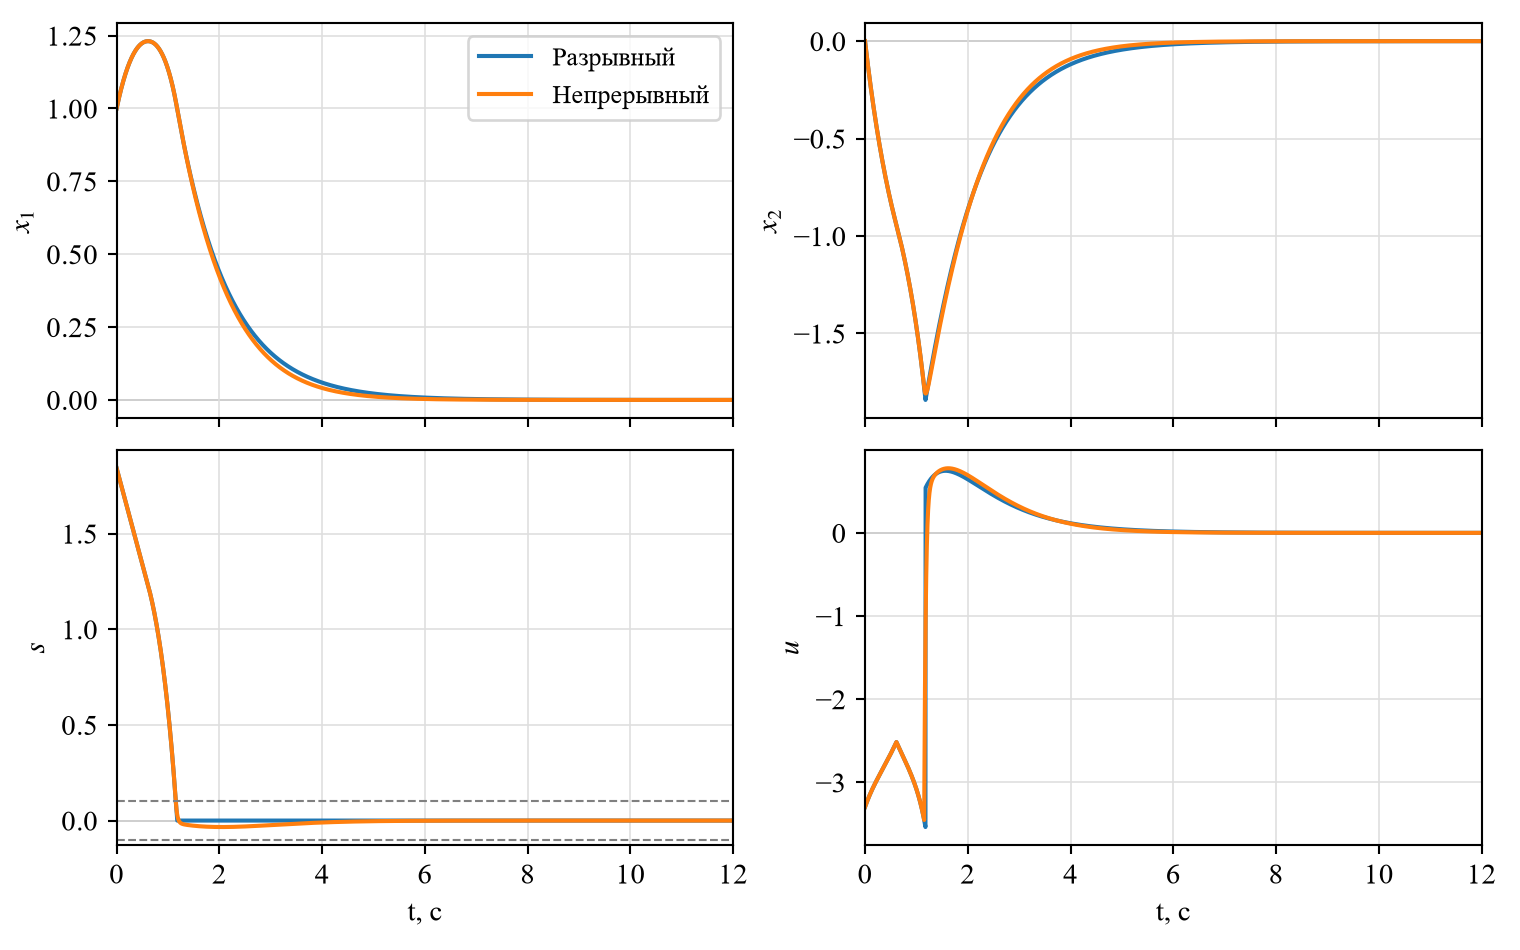
\includegraphics[width=0.95\textwidth]{../lab5/tex/images/task1_comparison.png}
 \caption{Первая система работы 5 Разрывный и непрерывный законы}
\end{guidefigure}

\subsection{Работа 5 Вторая система и робастный наклон поверхности}
\addition Для системы
\[
 \dot x_1=x_2+a_1x_1\sin x_1,\qquad
 \dot x_2=a_2x_1x_2+3u,\qquad a_1,a_2\in[0,2]
\]
параметр $a_1$ уже занят неизвестным коэффициентом объекта.
Поэтому наклон поверхности задаём непосредственно числом:
\[
 s=3x_1+x_2.
\]
На $s=0$ выполняется
\[
 \dot x_1=(-3+a_1\sin x_1)x_1,\qquad
 x_1\dot x_1\le-(3-2)x_1^2=-x_1^2.
\]
Число $3$ выбрано больше верхней границы $a_1$. Например,
наивная поверхность $s=x_1+x_2=0$ при $a_1=2$ допускает ненулевое
равновесие $x_1=\pi/6$, поскольку $-1+2\sin(\pi/6)=0$.
Она не обеспечивает требуемое глобальное притяжение к нулю.

Для выбранной поверхности
\[
 \dot s=3x_2+3a_1x_1\sin x_1+a_2x_1x_2+3u.
\]
Нормируем неопределённость на известный входной коэффициент $3$:
\[
 \left|x_2+a_1x_1\sin x_1+\frac{a_2}{3}x_1x_2\right|
 \le|x_2|+2|x_1\sin x_1|+\frac23|x_1x_2|=\varrho(x).
\]
Отсюда закон и его оценка:
\[
 \beta=\varrho+1,\qquad u=-\beta\sgn s,\qquad
 V=\frac{s^2}{2},\quad \dot V\le-3|s|,\quad
 t_*\le\frac{|s(0)|}{3}.
\]
До достижения $\frac{d}{dt}|x_1|\le-|x_1|+|s|$ почти всюду,
что даёт ограниченность. После достижения
\[
 |x_1(t)|\le|x_1(t_*)|e^{-(t-t_*)},\qquad x_2=-3x_1.
\]
Начало глобально асимптотически устойчиво для всех допустимых параметров.
Эквивалентный вход для отображения идеального скольжения равен
\[
 u_{eq}=3x_1-a_1x_1\sin x_1+a_2x_1^2.
\]
Последнее слагаемое положительно: оно получается из
$-a_2x_1x_2/3$ при $x_2=-3x_1$.
При $a_1=a_2=2$, $x(0)=(1{,}5;0)^T$ моделирование даёт
$t_*\approx0{,}163$ с, затем оба состояния сходятся к нулю.

\subsection{Работа 5 Непрерывное управление маятником}
\addition Задано уравнение
\[
 ml\ddot\theta+mg\sin\theta+kl\dot\theta
 =\frac{T}{l}+mh(t)\cos\theta,
\]
\[
 l\in[0{,}8;1],\quad m\in[0{,}5;1],\quad
 k\in[0{,}1;0{,}2],\quad |h(t)|\le0{,}5,\quad g=9{,}81.
\]
В этой задаче $g$ --- ускорение свободного падения, $h(t)$ --- внешнее
ускорение, $T$ --- управляющий момент. Это физические обозначения задания,
а не функции $g(x),h(x)$ из общего шаблона~\eqref{eq:sm-general}.
После деления на $ml$ имеем
\[
 \ddot\theta=-\frac gl\sin\theta-\frac km\dot\theta
             +\frac{T}{ml^2}+\frac{h(t)}l\cos\theta.
\]
Положим $x_1=\theta$, $x_2=\dot\theta$, $s=x_1+x_2$.
Умножая $\dot s$ на $ml^2$, получаем
\[
 ml^2\dot s=l^2(m-k)x_2-mgl\sin x_1+mlh(t)\cos x_1+T.
\]
Границы параметров дают $|l^2(m-k)|\le0{,}9$, $mgl\le9{,}81$,
$ml|h|\le0{,}5$. Поэтому подходит
\begin{equation}
 \varrho(x)=0{,}9|x_2|+9{,}81|\sin x_1|+0{,}5|\cos x_1|,
 \qquad T=-(\varrho+1)\sat(s/\varepsilon).
 \label{eq:pendulum-sat}
\end{equation}
Закон использует только угол, скорость и известные границы. Значения
$m,l,k$ и $h(t)$ ему не требуются.
При $|s|\ge\varepsilon$ для $V=s^2/2$ выполняется
\[
 \dot V\le-\frac{|s|}{ml^2}\le-|s|,
 \qquad t_\varepsilon\le\max\{|s(0)|-\varepsilon,0\},
\]
поскольку $ml^2\le1$. Полоса инвариантна. Для
$\tau=t-t_\varepsilon\ge0$ из $\dot\theta=-\theta+s$ следует
\[
 |\theta(t)|\le e^{-\tau}|\theta(t_\varepsilon)|
 +\varepsilon(1-e^{-\tau}),
\]
\[
 \limsup_{t\to\infty}|\theta(t)|\le\varepsilon,\qquad
 \limsup_{t\to\infty}|\dot\theta(t)|\le2\varepsilon.
\]
До входа $s$ ограничен, следовательно, угол и скорость также ограничены.
Гарантия глобальна по начальным условиям. При $\varepsilon=0{,}05$
предельные оценки составляют $0{,}05$ рад и $0{,}1$ рад/с.
Угол не обязан сразу после достижения полосы попасть в интервал
$[-\varepsilon,\varepsilon]$: в оценке ещё присутствует затухающая
зависимость от начального угла.

\subsubsection{Почему здесь гарантируется окрестность}

В состоянии $\theta=\dot\theta=0$ уравнение равновесия требует
\[
 T(0,0)=-mlh(t).
\]
Один непрерывный статический закон $T=T(\theta,\dot\theta)$ не может иметь
в нуле разные значения для всех неизвестных $h(t)$. При насыщении
в~\eqref{eq:pendulum-sat} $T(0,0)=0$, поэтому ненулевое ускорение
может вывести маятник из точного нуля. Для этой задачи корректно заявлять
глобальную \emph{практическую} стабилизацию, то есть достижение малой
заданной окрестности. Это принципиально отличается от первой системы,
в которой неопределённые слагаемые исчезают в нуле и точная сходимость
доказана отдельно.

\clearpage
\section{Адаптивное и робастное управление}
\label{sec:adaptive}

\subsection{Адаптация усиления при неизвестном параметре}
\lecture{L6}{15--17}

Адаптивный регулятор изменяет свои параметры во времени, используя измерения
объекта. В примере лекции требуется стабилизировать скалярную систему
\[
 \dot x=ax+u,\qquad a=-a_0+\Delta a,\qquad a_0>0,
\]
где $\Delta a$ --- неизвестное постоянное число. Если бы $a$ было известно,
можно было бы сразу выбрать достаточно сильную отрицательную обратную связь.
Адаптивный закон позволяет обойтись без известной верхней границы $\Delta a$:
\begin{equation}
 u=-c(t)x,\qquad \dot c=\gamma x^2,\qquad \gamma>0.
 \label{eq:adaptive-law}
\end{equation}
Здесь $c$ --- состояние регулятора, а $\gamma$ --- коэффициент скорости
адаптации. Это не входной коэффициент $\gamma(x)$ из линеаризации обратной
связью: обозначение используется в другом локальном контексте лекции.

Подстановка закона даёт
\[
 \dot x=-a_0x-(c-\Delta a)x.
\]
Вводится функция Ляпунова для состояния и отклонения усиления:
\[
 V(x,c)=\frac{x^2}{2}+\frac{(c-\Delta a)^2}{2\gamma}.
\]
Параметр $\Delta a$ входит в доказательство, но не требуется для вычисления
управления или $\dot c$. Поскольку $\Delta a$ постоянно,
\begin{align*}
 \dot V&=x[-a_0x-(c-\Delta a)x]
       +\frac{c-\Delta a}{\gamma}\dot c\\
 &=-a_0x^2+\frac{c-\Delta a}{\gamma}(\dot c-\gamma x^2)
 =-a_0x^2\le0.
\end{align*}
Правило адаптации выбрано именно для сокращения неизвестного смешанного
слагаемого. Если $x\ne0$, усиление $c$ увеличивается. Когда ошибка уменьшается,
скорость адаптации также уменьшается. В иллюстрации лекции используется
частный случай $\gamma=1$, то есть $\dot c=x^2$.

\addition Из $V(t)\le V(0)$ следуют ограниченность $x$ и $c$ и полнота
решения. В множестве $\dot V=0$ имеем $x=0$; оно инвариантно при любом
постоянном $c$. По принципу ЛаСалля $x(t)\to0$. В силу $\dot c\ge0$ и
ограниченности $c$ имеет конечный предел. Но из доказательства не следует
$c(t)\to\Delta a$: на $x=0$ адаптация останавливается при любом значении
усиления. Стабилизация состояния и идентификация неизвестного параметра
не являются одним и тем же результатом.

Также неверно утверждать, что $\dot V<0$ для любого ненулевого
$(x,c-\Delta a)$. При $x=0$, $c\ne\Delta a$ производная равна нулю.
Поэтому строгий вывод относится к сходимости $x$, а не к асимптотической
устойчивости единственной точки $(0,\Delta a)$ расширенной системы.

\subsection{Адаптивный закон с релейной составляющей}
\lecture{L6}{18--19}

Лекция дополняет управление постоянным релейным усилением:
\[
 u=-cx-d\sgn x,\qquad d>0,\qquad \dot c=\gamma x^2.
\]
Для прежней функции Ляпунова получается
\[
 \dot V=-a_0x^2-dx\sgn x=-a_0x^2-d|x|\le0.
\]
Квадратичное слагаемое отвечает за обычное затухание, дополнительное
$-d|x|$ усиливает притяжение при малых ненулевых $x$.
Закон опять не использует $\Delta a$. При $x=0$ разрыв трактуется
как в разделе о скользящем режиме.

\addition Нельзя автоматически подставить полную $V(x,c)$ в формулу
конечного времени с $\dot V\le-k\sqrt V$: величина $V$ включает ошибку
усиления, которая может остаться ненулевой после $x=0$.
Наличие в $\dot V$ слагаемого $-|x|$ не является само по себе доказательством
конечного времени обращения всей расширенной функции $V$ в нуль.

\subsection{Робастное усиление при известном интервале параметра}
\lecture{L6}{20--21}

Робастный регулятор использует известное множество возможных параметров
и обеспечивает результат для любого элемента этого множества.
Для $\dot x=ax+u$ пусть
\[
 \underline a\le a\le\overline a.
\]
Выбираем постоянное усиление
\[
 u=-kx,\qquad k>\overline a.
\]
Тогда $\dot x=-(k-a)x$, а решение удовлетворяет равномерной оценке
\[
 |x(t)|=|x(0)|e^{-(k-a)t}
 \le|x(0)|e^{-(k-\overline a)t}.
\]
Доказана глобальная экспоненциальная устойчивость для всего интервала.
В примере лекции указан закон $u=-3x$; он подходит, когда известная верхняя
граница $a$ строго меньше $3$. Для произвольного неизвестного и ничем
не ограниченного $a$ такое фиксированное усиление гарантии не даёт.

В отличие от адаптации здесь нет собственного состояния регулятора:
усиление выбирается один раз по худшему допустимому случаю. Этот выбор
может быть консервативным, зато доказательство сразу охватывает весь
заданный диапазон.

\subsection{Робастное подавление ограниченного возмущения}
\lecture{L6}{22--25}

Теперь объект имеет вид
\[
 \dot x=ax+u+f(t),\qquad
 a\in[\underline a,\overline a],\qquad |f(t)|\le\alpha.
\]
При одном $u=-kx$ постоянное $f$ оставило бы установившееся смещение.
В лекции выбирается
\begin{equation}
 u=-kx-k_0\sgn x,\qquad k>\overline a,\quad k_0>\alpha.
 \label{eq:robust-scalar}
\end{equation}
Для $V=x^2/2$ имеем
\begin{align*}
 \dot V&=-(k-a)x^2-k_0|x|+xf(t)\\
 &\le-(k-\overline a)x^2-(k_0-\alpha)|x|.
\end{align*}
Неизвестное возмущение оценивается по модулю. Строгий запас
$k_0-\alpha>0$ сохраняет притяжение даже при наихудшем знаке $f$.
Поскольку возмущение входит в тот же канал, что и управление, релейная
часть способна поддерживать идеальное скольжение в нуле.

\addition Для $x\ne0$ из этой же оценки следует
\[
 \frac{d}{dt}|x|\le-(k-\overline a)|x|-(k_0-\alpha)
 \le-(k_0-\alpha).
\]
Следовательно, в смысле Филиппова нуль достигается за
$t_*\le|x(0)|/(k_0-\alpha)$.
В численной иллюстрации лекции
\[
 u=-3x-4\sgn x,\qquad f(t)=2\sin50t.
\]
Здесь $\alpha=2$, запас реле равен $2$, а условие линейной части ---
$\overline a<3$. Возмущение быстро меняется, но для оценки важна его
амплитуда, а не возможность вычислить его мгновенное значение.
Идеальная оценка времени даёт $t_*\le|x(0)|/2$.

Если заменить знак насыщением, компенсация в самом нуле становится
однозначной и нулевой; произвольное ненулевое $f$ уже может вывести систему
из нуля. Тогда необходимо заново получить оценку окрестности или доказать
точную сходимость при дополнительных свойствах неопределённости.
Именно это различие используется при разборе двух непрерывных регуляторов
работы 5.

\subsection{Как сопоставить подходы на защите}

\begin{center}
\begin{tabularx}{\textwidth}{@{}lYY@{}}
\toprule
Подход & Что заранее известно & Как используется неопределённость\\
\midrule
Точная компенсация & Нелинейности и коэффициент входа & Вычисляются непосредственно в законе\\
Робастное усиление & Гарантированные границы & Выбирается запас для худшего случая\\
Скользящий режим & Знак входа и оценка нормированной ошибки & Релейная часть превосходит эту оценку\\
Адаптация & Структура модели и доступные измерения & Усиление изменяется по измеряемой ошибке\\
\bottomrule
\end{tabularx}
\end{center}
Эти подходы могут сочетаться: достаточно точная номинальная компенсация
может уменьшить релейную часть, адаптация изменяет усиление,
насыщение делает сигнал непрерывным.
Но для каждой полученной комбинации требуется своё доказательство;
свойства одного составляющего метода нельзя переносить на весь контур
без проверки.

\clearpage
\section{Подготовка к устной защите}
\label{sec:defense}

\subsection{Как последовательно объяснить свой регулятор}

Для каждого пункта работы полезно восстановить одно связное доказательство.
Начните с модели, измеряемых переменных и целевого равновесия. Затем
объясните, какая идея метода определила замену координат или поверхность.
Выведите управление из нужной динамики и только после этого сформулируйте
результат об устойчивости. В конце назовите область определения закона,
необходимые предположения и смысл численного опыта.

На защите важно уметь переходить в обе стороны: из формулы закона получить
уравнение замкнутой системы и из желаемого уравнения снова вывести закон.
Это сразу выявляет потерянный знак, пропущенную производную или неизвестный
параметр, случайно попавший в реализуемый регулятор.

\subsection{Общие вопросы}

\begin{enumerate}
\item \textbf{Чем устойчивость отличается от притяжения?}
Устойчивость удерживает близкие начальные состояния близко к равновесию.
Притяжение означает сходимость к равновесию. Асимптотическая устойчивость
требует обоих свойств; экспоненциальная дополнительно задаёт скорость
$\norm{x(t)}\le M e^{-\lambda(t-t_0)}\norm{x(t_0)}$.

\item \textbf{Почему $\dot V\le0$ недостаточно для асимптотической устойчивости?}
Вне нуля могут существовать траектории с постоянной $V$. Нужно исследовать
наибольшее инвариантное множество в $\{\dot V=0\}$, например по ЛаСаллю.
При прямой равновесий получается устойчивость множества, но не притяжение
к одной выбранной точке этой прямой.

\item \textbf{Что добавляет радиальная неограниченность?}
Она делает подуровни $V$ ограниченными и позволяет переносить локальное
рассуждение об убывании на любые начальные состояния, если условия на
производную выполняются глобально. Также нужна определённость $V$
относительно правильного равновесия и полнота решений.

\item \textbf{Гурвицева матрица всегда даёт глобальный результат?}
Для линейной системы --- да. Если это только якобиан нелинейной системы
в равновесии, результат локальный. Глобальный вывод после точной
линеаризации требует глобальной замены координат и глобально определённой
обратной связи.

\item \textbf{Сохраняется ли глобальная экспоненциальная оценка при любой замене координат?}
Глобальная асимптотическая устойчивость сохраняется при глобальном
диффеоморфизме, переводящем равновесие в нуль. Для той же глобальной
экспоненциальной оценки по исходной норме нужны дополнительные глобальные
сравнения норм, например двусторонние липшицевы оценки преобразования.

\item \textbf{Чем отличаются finite-time и fixed-time?}
При finite-time время достижения конечно для каждого начального состояния,
но может расти с его величиной. При fixed-time имеется общая верхняя граница
времени для всех начальных состояний. Конечное время достижения поверхности
скольжения не означает конечного времени достижения начала координат.
\end{enumerate}

\subsection{Вопросы по работе 3}

\begin{enumerate}[resume]
\item \textbf{Что такое относительная степень $\rho$?}
Это номер первой производной выхода, содержащей управление с ненулевым
коэффициентом. Предыдущие коэффициенты $L_gL_f^{i-1}h$ должны равняться нулю
в рассматриваемой области, а последний $L_gL_f^{\rho-1}h$ --- не обращаться
в нуль. Одной проверки в произвольной отдельно взятой точке недостаточно
для утверждения об области.

\item \textbf{Почему внутренние координаты выбираются из $L_g\varphi_i=0$?}
Тогда $\dot\eta_i=L_f\varphi_i$ не содержит непосредственного слагаемого
с $u$. Но управление по-прежнему влияет на внутреннюю динамику через
внешние координаты $\xi$; внутренние переменные не обязательно автономны
при ненулевом выходе.

\item \textbf{Почему одного ненулевого якобиана недостаточно для глобальности?}
Теорема об обратной функции даёт локальную обратимость.
Разные исходные точки всё ещё могут переходить в одинаковые новые
координаты. Нужны инъективность и подходящий глобальный обратный переход;
в задаче 4 две ветви $x_3>0$ и $x_3<0$ имеют одно и то же изображение.

\item \textbf{Что такое нуль-динамика?}
Это движение внутренних координат при поддержании выхода и его нужных
производных тождественно нулевыми. В нормальной форме она равна
$\dot\eta=f_0(\eta,0)$. При этом вход обычно равен компенсации
$u=\alpha(x)$, а не обязательно нулю.

\item \textbf{Почему система 1 не минимально-фазовая?}
Её нуль-динамика имеет собственные значения $0,-2$ и прямую равновесий
$\eta_1=\eta_2$. Составляющая вдоль этой прямой не затухает.
По лекционному определению нужна асимптотическая устойчивость нуль-динамики.

\item \textbf{Почему система 2 стабилизируется глобально?}
Замена $\eta=x_3-x_1^2/2$, $\xi_1=x_1$, $\xi_2=-x_1+x_2$
глобально обратима. При $u=x_1x_3-x_1$ вся система в новых координатах
линейна с полюсами $-2,-1,-1$. Устойчивость доказана для всех новых
координат, включая внутреннюю $\eta$.

\item \textbf{Как система 3 может иметь нулевой выход и расходящееся состояние?}
При $\xi_1(0)=\xi_2(0)=0$, $\eta(0)\ne0$ внешняя динамика остаётся нулевой,
а $x_3=\eta=\eta(0)e^t$. Линеаризующий вход компенсирует влияние $x_3$
на выход, но не устраняет неустойчивость самого $x_3$.

\item \textbf{Что особенного в системе 4?}
И коэффициент $L_gL_fh=x_3$, и определитель $DT=-x_3$ вырождаются на
$x_3=0$. На каждой ветви есть обратный корень
$x_3=\pm\sqrt{2(\xi_2-\eta)}$. Нуль-динамика приближается к границе
регулярной области, поэтому нельзя назвать преобразование и дробь
$(x_1+v)/x_3$ регулярными в предельной точке.

\item \textbf{Почему в системе 5 $K=(12,16,7)$, а не $(7,16,12)$?}
Для цепочки третьего порядка с $v=-k_1z_1-k_2z_2-k_3z_3$
характеристический полином равен $s^3+k_3s^2+k_2s+k_1$.
Он должен совпасть с $(s+2)^2(s+3)=s^3+7s^2+16s+12$.
После подстановки $z_3=x_3+x_1^2$ обязательно появляется член $-7x_1^2$.
\end{enumerate}

\subsection{Вопросы по работе 4}

\begin{enumerate}[resume]
\item \textbf{Что является виртуальным управлением?}
Это желаемое значение следующего состояния, например $x_2=\phi(x_1)$.
Его нельзя подать непосредственно на объект: физический вход управляет
производной следующего состояния. Поэтому вводится ошибка
$z_2=x_2-\phi$ и строится следующий шаг.

\item \textbf{Откуда берётся $\dot\phi$?}
Из дифференцирования ошибки: $\dot z=\dot\xi-\dot\phi$.
Это полная производная по исходной системе,
$\dot\phi=\sum_j(\partial\phi/\partial x_j)\dot x_j$.
Пропуск этого члена изменяет замкнутую динамику и разрушает сокращение
смешанных слагаемых в $\dot V_c$.

\item \textbf{Почему производные виртуальных управлений ещё являются обратной связью по состоянию?}
В строгой треугольной структуре $\phi_i$ зависит только от первых $i$
координат, производные которых до последнего шага не содержат настоящего
входа $u$. Поэтому $\dot\phi_i$ вычисляется через измеренное состояние.
Это нужно проверить, а не использовать как безусловное свойство любой системы.

\item \textbf{Что удерживает третью систему в ненулевой точке?}
Для неё $x_{ss}=(0,1,0,0)^T$, \mbox{$u_{ss}=0$}. В нуле $\dot x_1=1$,
поэтому нуль не равновесие. В целевой точке $\cos0-x_2=1-1=0$,
а остальные производные также нулевые. Ошибки бэкстеппинга обращаются
в нуль именно в этой точке.

\item \textbf{Почему в производной $\phi_3$ нужен дополнительный член от знаменателя?}
При $\phi_3=N/g_2$, $g_2=2-\sin x_3$,
\[
 \frac{\partial\phi_3}{\partial x_3}
 =\frac{\partial N/\partial x_3}{g_2}
  +\frac{N\cos x_3}{g_2^2}.
\]
Плюс появляется потому, что $\partial g_2/\partial x_3=-\cos x_3$.
Граница $g_2\ge1$ гарантирует отсутствие сингулярности всех шагов.
\end{enumerate}

\subsection{Вопросы по работе 5}

\begin{enumerate}[resume]
\item \textbf{Что выбирается первым --- усиление или поверхность?}
Сначала поверхность, на которой движение должно быть устойчивым, затем
усиление, обеспечивающее её достижение. В первой системе
$s=x_1+x_2+\sin x_1$, во второй $s=3x_1+x_2$; эти поверхности выбраны
из разных первых уравнений объектов.

\item \textbf{Что означает $\beta_0>0$?}
Это строгий запас над оценкой неопределённости:
$\beta\ge\varrho+\beta_0$. Он даёт
$\frac{d}{dt}|s|\le-g_0\beta_0$ и конечное время достижения.
Если убрать запас, простого строгого неравенства для конечного времени
уже может не быть.

\item \textbf{Почему нельзя реализовать идеальное скольжение простой подстановкой $\sgn0=0$?}
В нуле поверхности требуется эквивалентный вход, компенсирующий дрейф.
В модели Филиппова он выбирается из интервала значений реле.
Обычное нулевое значение знака в одной точке этого не описывает.

\item \textbf{Почему непрерывность не означает дифференцируемость?}
Функция $\sat(s/\varepsilon)$ непрерывна, но её производная меняется скачком
при $|s|=\varepsilon$. Регулятор непрерывный; называть его обязательно
гладким в смысле $C^1$ было бы неверно.

\item \textbf{Почему насыщенный регулятор системы 1 приводит точно к нулю?}
После достижения полосы отдельная полная функция
$V_c=(x_1^2+s^2)/2$ удовлетворяет $\dot V_c\le-V_c$ при
$0<\varepsilon\le1/4$. Неопределённость исчезает в нуле,
а выбранное усиление перекрывает смешанные члены.
Это специальный результат данной системы.

\item \textbf{Почему для маятника остаётся окрестность?}
При ненулевом неизвестном $h(t)$ в самом нуле требуется неизвестный
момент $-mlh(t)$. Непрерывный статический закон насыщения в нуле даёт
единственное значение $0$. Поэтому доказаны оценки
$\limsup|\theta|\le\varepsilon$ и
$\limsup|\dot\theta|\le2\varepsilon$.

\item \textbf{Почему усиление адаптации не обязательно сходится к неизвестному параметру?}
Для $\dot c=\gamma x^2$ при $x=0$ изменение $c$ прекращается при любом его
значении. Функция Ляпунова доказывает $x\to0$ и ограниченность $c$,
а не идентификацию $\Delta a$.
\end{enumerate}

\subsection{Как объяснить численное моделирование}
\addition В работах 4 и 5 используется метод Рунге-Кутты четвёртого порядка.
Для автономной правой части $F$ и шага $h$ один шаг имеет вид
\[
 \begin{aligned}
 k_1&=F(x_i),& k_2&=F(x_i+hk_1/2),\\
 k_3&=F(x_i+hk_2/2),& k_4&=F(x_i+hk_3),\\
 x_{i+1}&=x_i+\frac h6(k_1+2k_2+2k_3+k_4).
 \end{aligned}
\]
В работе 4 заданы $h=0{,}001$ с, $t\in[0,10]$ с,
$x(0)=(1;-0{,}5)^T$ для первых двух систем и
$x(0)=(0{,}5;1;-0{,}5;0{,}25)^T$ для третьей.
Правая часть на каждом этапе вычисляется вместе с обратной связью
в промежуточном состоянии. Для третьей системы отображаются
$x_1$, $x_2-1$, $x_3$, $x_4$, а не требование занулить все исходные координаты.

В работе 5 используются тот же шаг, интервал $[0,12]$ с,
параметры $\theta_1=1$, $\theta_2=-1$, $a_1=a_2=2$ и начальные
состояния $(1,0)^T$, $(1{,}5;0)^T$ соответственно. Эти числа известны
модели объекта, а робастный закон использует только границы и состояние.
Для непрерывного закона взято $\varepsilon=0{,}1$.

Разрывная динамика интегрируется до пересечения $s=0$.
В сокращённом скрипте момент пересечения внутри шага оценивается линейной
интерполяцией значения $s$:
\[
 \tau\approx h\frac{s_i}{s_i-s_{i+1}},\qquad 0\le\tau\le h.
\]
После него интегрируется движение на поверхности и отображается
эквивалентное управление. Для непрерывного закона насыщение вычисляется
непосредственно на каждом этапе. Поэтому отсутствие частых переключений
на идеальном графике реле не является доказательством отсутствия chattering
у реального привода.

Один численный опыт подтверждает поведение выбранной модели при конкретных
начальных условиях и параметрах. Гарантия для всех допустимых параметров
и всех начальных состояний обеспечивается аналитическими оценками,
а не самим видом графика.

\end{document}
